
\PassOptionsToPackage{table}{xcolor}
\documentclass[letterpaper]{article} % DO NOT CHANGE THIS
\usepackage[submission]{aaai2026}  % DO NOT CHANGE THIS
% \usepackage{aaai2026}
\usepackage{times}  % DO NOT CHANGE THIS
\usepackage{helvet}  % DO NOT CHANGE THIS
\usepackage{courier}  % DO NOT CHANGE THIS
\usepackage[hyphens]{url}  % DO NOT CHANGE THIS
\usepackage{graphicx} % DO NOT CHANGE THIS
\urlstyle{rm} % DO NOT CHANGE THIS
\def\UrlFont{\rm}  % DO NOT CHANGE THIS
\usepackage{natbib}  % DO NOT CHANGE THIS AND DO NOT ADD ANY OPTIONS TO IT
\usepackage{caption} % DO NOT CHANGE THIS AND DO NOT ADD ANY OPTIONS TO IT
\frenchspacing  % DO NOT CHANGE THIS
\setlength{\pdfpagewidth}{8.5in} % DO NOT CHANGE THIS
\setlength{\pdfpageheight}{11in} % DO NOT CHANGE THIS
%
% These are recommended to typeset algorithms but not required. See the subsubsection on algorithms. Remove them if you don't have algorithms in your paper.
\usepackage{algorithm}
\usepackage{algorithmic}

% YipanWei Edited
\usepackage[table]{xcolor}
\usepackage{multirow}
\usepackage{arydshln}
\usepackage{placeins}

\definecolor{DarkGreen}{RGB}{34,120,50}


\newcommand{\pub}[1]{{\color{gray}{\footnotesize{[{#1}]}}}}

\newcommand{\tworowbestreshl}[2]{%
\begin{tabular}{@{}c@{}}
{#1}  \\
{\small\color{DarkGreen}{$+$ \textbf{#2}}}
\end{tabular}%
}

%
% These are are recommended to typeset listings but not required. See the subsubsection on listing. Remove this block if you don't have listings in your paper.
\usepackage{newfloat}
\usepackage{listings}
\DeclareCaptionStyle{ruled}{labelfont=normalfont,labelsep=colon,strut=off} % DO NOT CHANGE THIS
\lstset{%
	basicstyle={\footnotesize\ttfamily},% footnotesize acceptable for monospace
	numbers=left,numberstyle=\footnotesize,xleftmargin=2em,% show line numbers, remove this entire line if you don't want the numbers.
	aboveskip=0pt,belowskip=0pt,%
	showstringspaces=false,tabsize=2,breaklines=true}
\floatstyle{ruled}
\newfloat{listing}{tb}{lst}{}
\floatname{listing}{Listing}
%
% Keep the \pdfinfo as shown here. There's no need
% for you to add the /Title and /Author tags.
\pdfinfo{
/TemplateVersion (2026.1)
}
\definecolor{LAMPYellow}{RGB}{255,220,112}
\definecolor{HeaderGray}{RGB}{235,235,235}
\definecolor{AvgBlue}{RGB}{226,241,255}
\definecolor{GainGreen}{RGB}{32,132,84}
\definecolor{DropRed}{RGB}{190,54,54}
\newcommand{\tblhead}[1]{\strut #1}
\newcommand{\lampcell}[1]{\begingroup\setlength{\fboxsep}{0pt}\colorbox{LAMPYellow}{\makebox[6.7em][c]{\rule[-1.12ex]{0pt}{4.45ex}\bfseries\boldmath #1}}\endgroup}
\newcommand{\avgcell}[1]{\begingroup\def\avgcontent{#1}\def\avgheader{Avg}\ifx\avgcontent\avgheader\bfseries #1\else\setlength{\fboxsep}{0pt}\colorbox{AvgBlue}{\makebox[3.55em][c]{\strut #1}}\fi\endgroup}
\newcommand{\metriclampcell}[1]{\begingroup\setlength{\fboxsep}{0pt}\colorbox{LAMPYellow}{\makebox[7.05em][c]{\rule[-0.96ex]{0pt}{3.95ex}\bfseries\boldmath #1}}\endgroup}
\newcommand{\lampband}{\noalign{\begingroup\color{LAMPYellow}\hrule height 3.35ex\endgroup\kern-3.35ex}}
\newcommand{\headband}{\noalign{\begingroup\color{HeaderGray}\hrule height 6.15ex\endgroup\kern-6.15ex}}
\newcommand{\gainup}[1]{\makebox[5.85em][l]{\textcolor{DropRed}{\(\uparrow\)#1}}}
\newcommand{\gaindown}[1]{\makebox[5.85em][l]{\textcolor{DropRed}{\(\downarrow\)#1}}}
\newcommand{\dropdown}[1]{\makebox[5.85em][l]{\textcolor{DropRed}{\(\downarrow\)#1}}}
\newcommand{\neutraldelta}[1]{\makebox[5.85em][l]{\textcolor{GainGreen}{#1}}}
\newcommand{\compactdrop}[1]{\textcolor{DropRed}{\(\downarrow\)#1}}
\newcommand{\compactgain}[1]{\textcolor{DropRed}{\(\uparrow\)#1}}
\newcommand{\compactneutral}[1]{\textcolor{GainGreen}{#1}}

\makeatletter
\setlength{\@fptop}{0pt}
\setlength{\@fpsep}{10pt}
\setlength{\@fpbot}{0pt}
\setlength{\@dblfptop}{0pt}
\setlength{\@dblfpsep}{10pt}
\setlength{\@dblfpbot}{0pt}
\makeatother
\setcounter{dbltopnumber}{4}
\renewcommand{\dbltopfraction}{0.99}
\renewcommand{\dblfloatpagefraction}{0.01}

% DISALLOWED PACKAGES
% \usepackage{authblk} -- This package is specifically forbidden
% \usepackage{balance} -- This package is specifically forbidden
% \usepackage{color (if used in text)
% \usepackage{CJK} -- This package is specifically forbidden
% \usepackage{float} -- This package is specifically forbidden
% \usepackage{flushend} -- This package is specifically forbidden
% \usepackage{fontenc} -- This package is specifically forbidden
% \usepackage{fullpage} -- This package is specifically forbidden
% \usepackage{geometry} -- This package is specifically forbidden
% \usepackage{grffile} -- This package is specifically forbidden
% \usepackage{hyperref} -- This package is specifically forbidden
% \usepackage{navigator} -- This package is specifically forbidden
% (or any other package that embeds links such as navigator or hyperref)
% \indentfirst} -- This package is specifically forbidden
% \layout} -- This package is specifically forbidden
% \multicol} -- This package is specifically forbidden
% \nameref} -- This package is specifically forbidden
% \usepackage{savetrees} -- This package is specifically forbidden
% \usepackage{setspace} -- This package is specifically forbidden
% \usepackage{stfloats} -- This package is specifically forbidden
% \usepackage{tabu} -- This package is specifically forbidden
% \usepackage{titlesec} -- This package is specifically forbidden
% \usepackage{tocbibind} -- This package is specifically forbidden
% \usepackage{ulem} -- This package is specifically forbidden
% \usepackage{wrapfig} -- This package is specifically forbidden
% DISALLOWED COMMANDS
% \nocopyright -- Your paper will not be published if you use this command
% \addtolength -- This command may not be used
% \balance -- This command may not be used
% \baselinestretch -- Your paper will not be published if you use this command
% \clearpage -- No page breaks of any kind may be used for the final version of your paper
% \columnsep -- This command may not be used
% \newpage -- No page breaks of any kind may be used for the final version of your paper
% \pagebreak -- No page breaks of any kind may be used for the final version of your paperr
% \pagestyle -- This command may not be used
% \tiny -- This is not an acceptable font size.
% \vspace{- -- No negative value may be used in proximity of a caption, figure, table, section, subsection, subsubsection, or reference
% \vskip{- -- No negative value may be used to alter spacing above or below a caption, figure, table, section, subsection, subsubsection, or reference

\setcounter{secnumdepth}{0} %May be changed to 1 or 2 if section numbers are desired.

% The file aaai2026.sty is the style file for AAAI Press
% proceedings, working notes, and technical reports.
%


%Example, Multiple Authors, ->> remove \iffalse,\fi and place them surrounding AAAI title to use it
\title{LAMP-Merge: Long-tail-Aware Medical Prototype Merging for One-shot Asynchronous Clinical Models}
\author {
    Wenjin Hu\equalcontrib\textsuperscript{\rm 1},
    Yipan Wei\equalcontrib\textsuperscript{\rm 1},
    Yapeng Li\textsuperscript{\rm 1},
    Zengmao Wang\textsuperscript{\rm 1} ,
    Bo Du\textsuperscript{\rm 1}
}

\affiliations {
    \textsuperscript{\rm 1}School of Computer Science, Wuhan University,
    Wuhan, Hubei, China\\
    wenjinhu@whu.edu.cn, yipanwei@whu.edu.cn,
    yapengli@whu.edu.cn, dubo@whu.edu.cn,
    wangzengmao@whu.edu.cn
}





% REMOVE THIS: bibentry
% This is only needed to show inline citations in the guidelines document. You should not need it and can safely delete it.
% \usepackage{bibentry}
% END REMOVE bibentry

\begin{document}
\maketitle

\begin{abstract}
Model merging aims to integrate multiple independently trained local checkpoints into a unified global model, typically through general-purpose paradigms such as parameter interpolation, task-vector composition, or update-direction alignment. These methods implicitly assume that client models share relatively complete and comparable global discriminative structures. We argue that this assumption does not hold in medical settings, giving rise to two diagnostic-structure anomalies: (1)\textbf{ Aggregation-induced prediction collapse after merging}: When clients have incomplete diagnostic-class coverage, multiple locally effective models can be merged into a globally collapsed model whose predictive distribution concentrates on a small number of dominant classes. (2)\textbf{ Long-tailed medical prevalence cannot be ignored}. Majority classes in medical data often reflect genuine clinical prevalence rather than merely data noise. To address these challenges, we propose \textbf{LAMP-Merge}, which recasts medical model merging from global parameter interpolation as class-level diagnostic-evidence reconstruction. Through \textbf{diagnostic prototype reconstruction(DPR)} and \textbf{long-tail prevalence calibration(LPC)}, LAMP-Merge constructs a global diagnostic model without exposing raw medical images or requiring multi-round federated communication. Experiments on the Blood, Derma, Organ-C, Organ-S, and Ultrasound medical imaging datasets show that LAMP-Merge outperforms existing model-merging methods in most client-averaged settings while substantially mitigating prediction collapse.

% Index Terms:medical model merging, asynchronous fusion, predictive collapse, long-tail calibration, privacy-preserving learning
\end{abstract}


% Uncomment the following to link to your code, datasets, an extended version or similar.
% You must keep this block between (not within) the abstract and the main body of the paper.
% \begin{links}
%     \link{Code}{https://aaai.org/example/code}
%     \link{Datasets}{https://aaai.org/example/datasets}
%     \link{Extended version}{https://aaai.org/example/extended-version}
% \end{links}

\section{Introduction}

Federated learning~\cite{pmlr-v54-mcmahan17a,li2020fedprox,karimireddy2020scaffold,kairouz2021advances} and model merging~\cite{izmailov2018averaging,pmlr-v162-wortsman22a,ilharco2023editingmodelstaskarithmetic,yadav2023tiesmergingresolvinginterferencemerging} provide two important collaboration routes for privacy-sensitive multicenter medical intelligence. Federated learning enables hospitals to train collaboratively without sharing raw data~\cite{sheller2020federated,rieke2020future}, while model merging further reduces communication and optimization costs by integrating independently trained local models after training~\cite{ainsworth2023gitrebasinmergingmodels,stoica2024zipit,wu_parameter_2025}. These paradigms are particularly attractive for \textbf{medical imaging}, because a single hospital rarely covers the full disease spectrum, while privacy regulations and device heterogeneity make centralizing raw medical images difficult ~\cite{kaissis2020secure,bonawitz2019towards,abadi2016deep}.

\begin{figure}[!t]
    \centering
    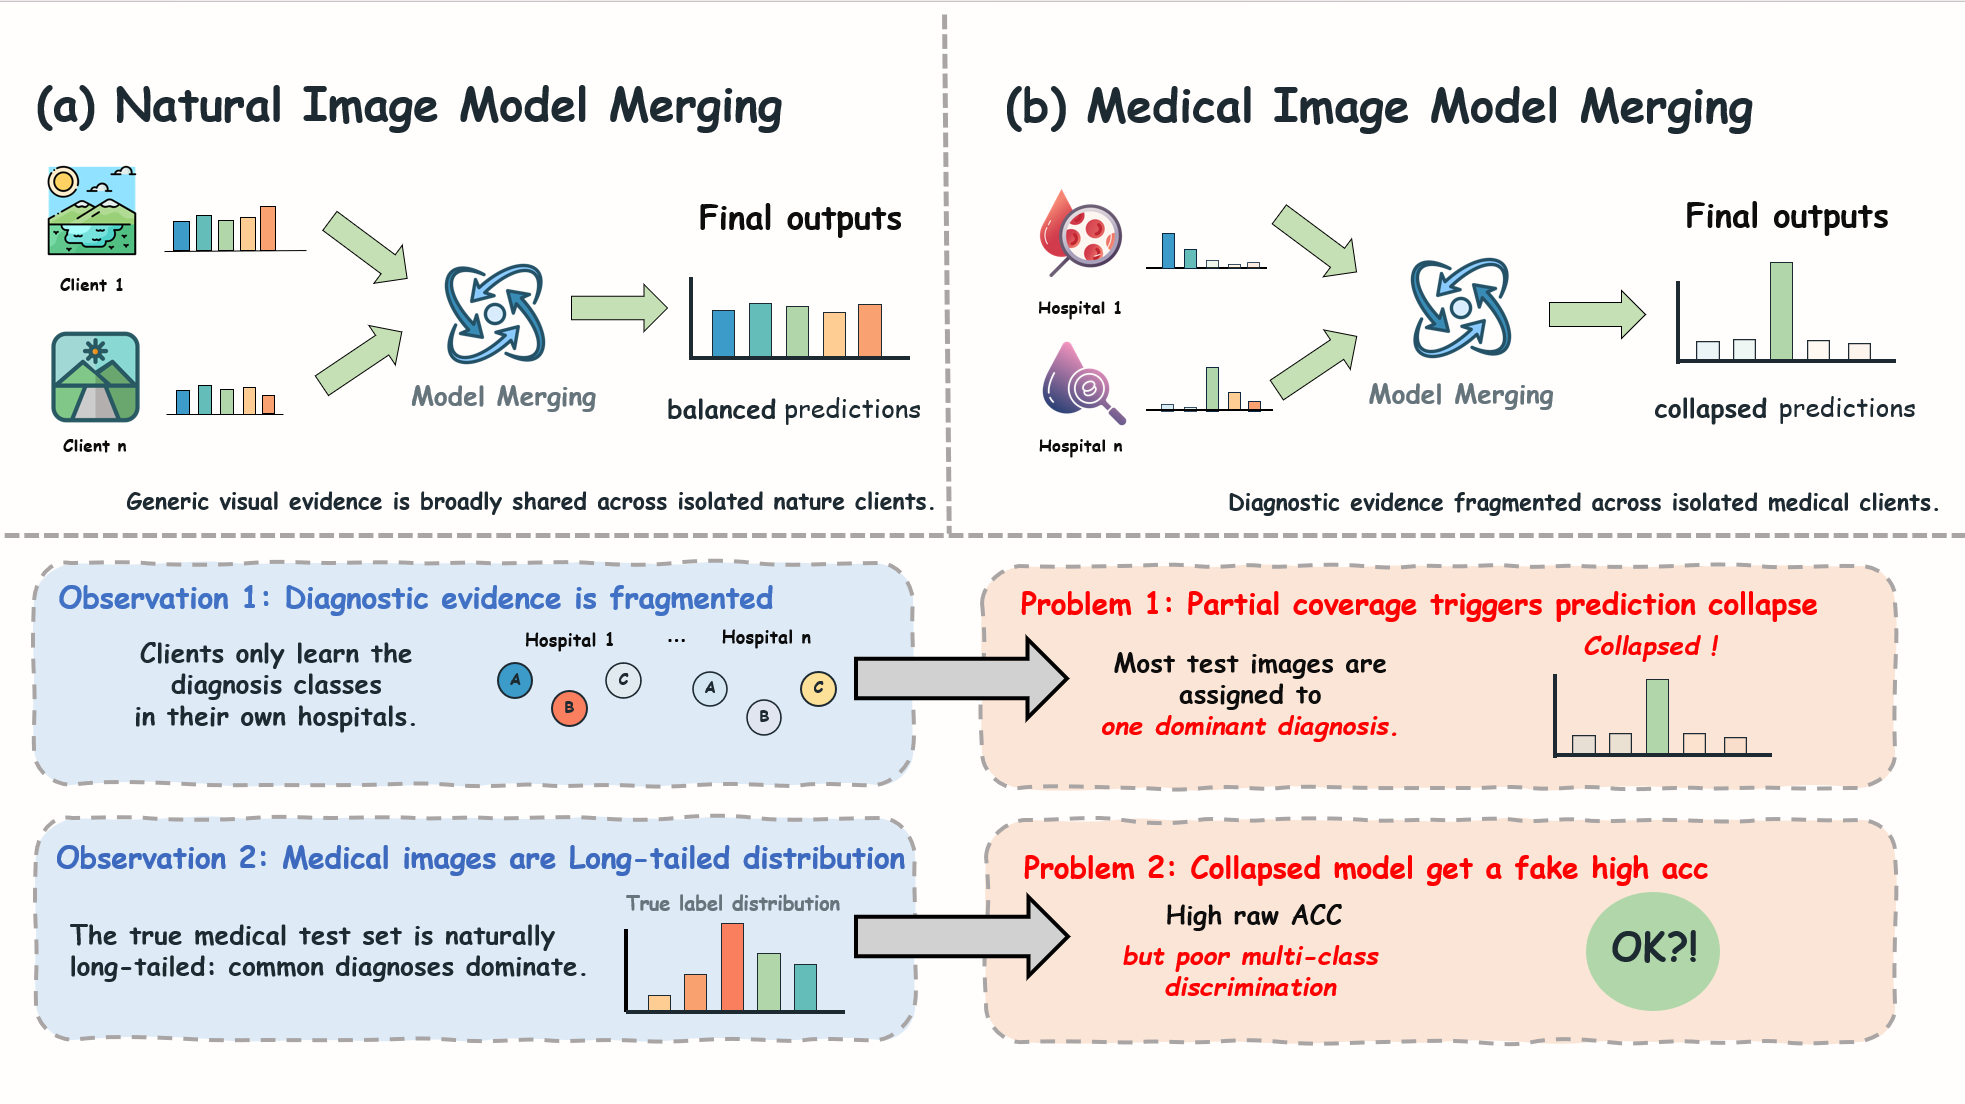
\includegraphics[width=0.96\linewidth]{figures/intro.png}
    \caption{\textbf{Motivation.} Unlike natural-image clients that share overlapping visual evidence, medical clients each observe only part of the diagnostic space, so parameter-level merging collapses the global model onto a few dominant classes. This reflects two observations: diagnostic evidence is fragmented across isolated clients, and medical prevalence is long-tailed---under which a collapsed model can still report deceptively high accuracy.}
 
    \label{fig:intro-collapse}
\end{figure}

Despite their success on natural images and general visual tasks~\cite{izmailov2018averaging,pmlr-v162-wortsman22a,ilharco2023editingmodelstaskarithmetic,entezari2022role,ainsworth2023gitrebasinmergingmodels}, transferring these paradigms to medical data remains challenging. A key reason is that general-purpose model merging implicitly assumes that different client checkpoints contain relatively complete and comparable \textbf{global discriminative structures}; local models are expected to align through parameter space, task-vector space, update signs, or curvature statistics~\cite{yadav2023tiesmergingresolvinginterferencemerging,yu2024languagemodelssupermario,wu_parameter_2025,jin2025datalessknowledgefusionmerging}. This assumption does not hold in medical scenarios. Medical centers differ not only in device domains but also in diagnostic-class availability: some centers may mainly cover common diseases or specific examination types, while having few rare-disease samples~\cite{9557808,10.1371/journal.pmed.1002683,li2021fedbn}. The resulting local models are not complete replicas of the global task, but \textbf{partial diagnostic experts} supported by locally observed diseases.

As illustrated in Fig.~\ref{fig:intro-collapse}, we summarize these challenges as two diagnostic-structure abnormalities in medical model merging:
\begin{itemize}
    \item \textbf{Diagnostic evidence fragmented across isolated medical clients.} Each client has reliable supervision only for observed classes; thus, a local model may be locally discriminative but still lack evidence for the full global diagnostic space~\cite{9557808,li2021fedbn}.
    \item \textbf{Long-tailed Medical Image Prevalence.} Medical image datasets naturally follow a long-tailed distribution: a few common diagnostic classes dominate the  samples, while rare classes are underrepresented~\cite{BUDA2018249,5597285}. Under this imbalanced class prior, a merged model collapsed to the majority class can still obtain high Accuracy despite lacking complete multi-class discrimination.
\end{itemize}

To address these issues, we propose \textbf{LAMP-Merge, a long-tail-aware medical prototype-merging method for single-shot asynchronous medical image model merging}. LAMP-Merge shifts the merge target from global parameter interpolation to \textbf{class-level diagnostic-evidence reconstruction}. The key idea is to use client-uploaded class-level statistics as a synchronization signal for the global diagnostic space, allowing the server to reconstruct a global diagnostic classifier without accessing raw medical images, using a server-side validation set, or conducting multi-round federated communication. Specifically, LAMP-Merge consists of two mechanisms: \textbf{diagnostic prototype reconstruction} aggregates reliable class-level evidence through prototypes in a shared reference feature space, and \textbf{long-tail prevalence calibration} injects a bounded prior bias from client-uploaded class counts, thereby mitigating prediction collapse while preserving clinically meaningful majority-class prevalence.

\begin{figure*}[!t]
    \centering
    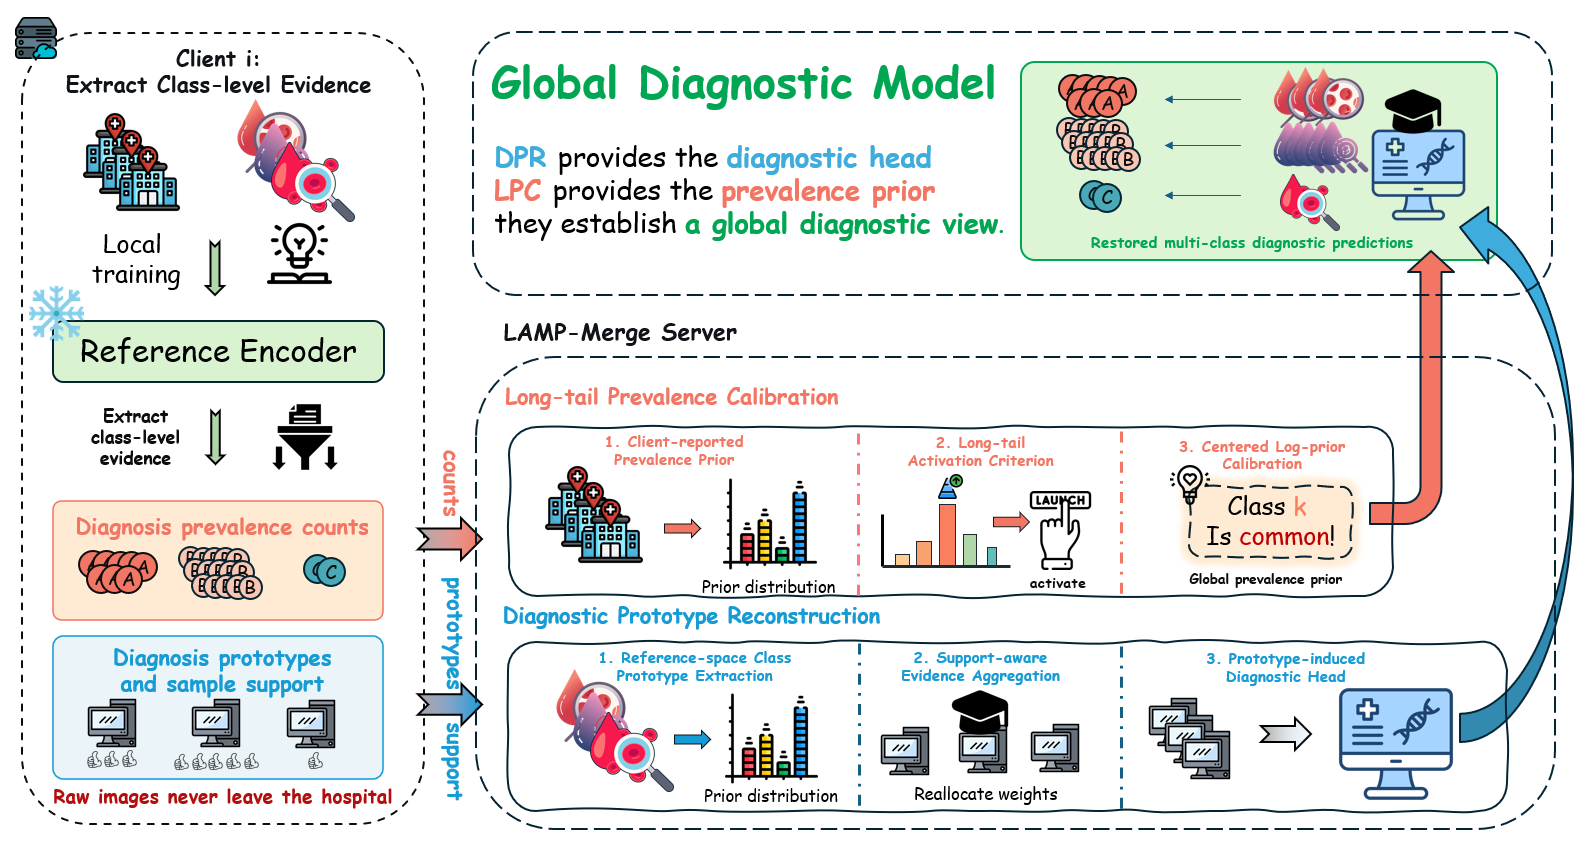
\includegraphics[width=0.92\textwidth,height=0.34\textheight]{figures/method.png}
    \caption{\textbf{Overview of LAMP-Merge.} Each hospital uploads only class-level statistics---reference-space prototypes with sample support and diagnosis prevalence counts---while raw images stay local. On the server, Diagnostic Prototype Reconstruction (DPR) aggregates the prototypes by support-aware weighting into a diagnostic head $\mathbf{w}_c$, and Long-tail Prevalence Calibration (LPC) adds a gated, bounded log-prior bias $b_c$, giving the scoring rule $\ell_c(x)=\mathbf{w}_c^{\top}\phi_0(T(x))+\mathbf{1}[r>\tau]\,b_c$ in a single-shot merge without raw-data sharing or federated rounds.}
 
    \label{fig_method}
\end{figure*}

Our main contributions are summarized as follows:
\begin{itemize}
    \item \textbf{Medical Merging Diagnosis.} We revisit model merging under single-shot asynchronous medical collaboration and identify limited local diagnostic coverage and aggregation-induced prediction collapse as two key abnormalities caused by medical class availability and long-tailed prevalence.
    \item \textbf{LAMP-Merge.} We propose a long-tail-aware medical prototype-merging method that reconstructs a global diagnostic classifier from client-side class prototypes and prevalence statistics without exposing raw images or requiring multi-round federated optimization.
    \item \textbf{Empirical Validation.} We conduct full-scope experiments on five medical image datasets, four vision-model families, three client-population sizes, and three non-IID skew levels, showing that LAMP-Merge consistently outperforms strong model-merging baselines and improves prediction-collapse diagnostics.
\end{itemize}

\section{Related Works}

\subsection{Model Merging}

Model-merging methods integrate independently trained checkpoints in parameter, task-vector, or geometric spaces. Weight averaging~\cite{izmailov2018averaging} and Model Soups~\cite{pmlr-v162-wortsman22a} directly interpolate parameters; permutation-aware matching~\cite{entezari2022role,ainsworth2023gitrebasinmergingmodels} aligns hidden-unit symmetries; ZipIt~\cite{stoica2024zipit} performs feature-level zipping; Task Arithmetic~\cite{ilharco2023editingmodelstaskarithmetic}, TIES-Merging~\cite{yadav2023tiesmergingresolvinginterferencemerging}, and DARE~\cite{yu2024languagemodelssupermario} manipulate task deltas and sign conflicts; Fisher merging~\cite{wu_parameter_2025}, RegMean~\cite{jin2025datalessknowledgefusionmerging}, Model Stock~\cite{jang2025modelstockneedjust}, Breadcrumbs~\cite{davari2024modelbreadcrumbsscalingmultitask}, Iso-C~\cite{marczak2025taskleftbehindisotropic}, FreeMerge~\cite{zheng2025freemergingfouriertransformefficient}, and RobustMerge~\cite{zeng2025robustmergeparameterefficientmodelmerging} introduce curvature, mean-statistic, subspace, frequency-domain, or robustness assumptions.

However, these methods share a class-agnostic merging interface: their variables are global parameters, task vectors, update signs, or geometric statistics rather than class-level diagnostic evidence. \textbf{They do not encode whether a client has reliable supervision for a specific medical class.} Under incomplete local class coverage and long-tailed prevalence, reliable class directions can be mixed with absent or conflicting directions from other clients, resulting in aggregation-induced prediction collapse\cite{BUDA2018249,10.1371/journal.pmed.1002683}.

One-shot clinical merging therefore requires class availability to be distinguished from model-wide parameter similarity.

\subsection{Medical Model Merging}

Medical fusion studies exploit domain structures such as irregular clinical time series, physiological sensor graphs, and image-EHR fusion. mTAN~\cite{shukla2021multitimeattentionnetworksirregularly}, Raindrop~\cite{zhang2022graphguidednetworkirregularlysampled}, and MedFuse~\cite{hayat2023medfusemultimodalfusionclinical} show that medical tasks benefit from modeling clinical sampling mechanisms, modality heterogeneity, and patient-level temporal relations.

However, their fusion objects are usually patient-level inputs, multimodal records, or clinical representations rather than independently trained image-classifier checkpoints. They often require patient samples, timestamps, electronic health records, or server-side validation feedback, which conflicts with common privacy constraints~\cite{kaissis2020secure,sheller2020federated,bonawitz2019towards}. MedMerge~\cite{11382027} is a relevant training-free medical knowledge-transfer framework, but it targets cross-modal adaptation for medical vision-language models rather than asynchronous checkpoint merging for the same classification task. \textbf{Thus, existing medical fusion routes are mismatched with our privacy and single-upload protocol constraints.} LAMP-Merge keeps the medical structure uploadable by using only locally computed class prototypes and prevalence counts.

\subsection{Federated Learning}

Federated and decentralized learning perform collaborative training through communication protocols. FedAvg~\cite{pmlr-v54-mcmahan17a} and its variants or medical deployments~\cite{li2020fedprox,karimireddy2020scaffold,li2021fedbn,kaissis_secure_2020,sheller2020federated,rieke2020future,kairouz2021advances} rely on repeated server-client updates; Swarm Learning~\cite{warnat-herresthal_swarm_2021} and Gossip Learning~\cite{hegedhus_gossip_2019} reduce centralization but still require participants to continue training, exchanging models, and optimizing from intermediate states.

However, our setting begins after local training has finished. Hospitals may not remain online, receive global checkpoints repeatedly, or run additional optimization rounds. \textbf{The bottleneck is therefore communication feasibility in addition to privacy.} LAMP-Merge requires one upload of a local model interface and class-level statistics, enabling the server to construct a unified diagnostic model without a multi-round feedback loop.

\section{Method}

In this section, we first formulate the diagnostic-structure pathologies exposed when generic model merging is applied to medical data, namely \textbf{limited local diagnostic coverage} and \textbf{aggregation-induced prediction collapse}. To correct these intrinsic mismatches, we propose \textbf{LAMP-Merge}, a two-stage framework composed of \textbf{DPR} and \textbf{LPC}, as shown in Fig.~\ref{fig_method}.

\subsection{Preliminaries}

\subsubsection{Problem Formulation.}

Assume $K$ medical clients. Client $i$ owns a private labeled dataset $D_i=\{(x,y)\}$ drawn from a class-skewed medical distribution over $C$ diagnosis classes. Let $D_{i,c}$ denote the subset of client $i$ belonging to diagnosis class $c$. In medical partitions, $D_{i,c}$ can be empty for many classes; therefore, client $i$ has reliable supervision only for its observed classes. The goal is to construct a global diagnostic model under this partial and heterogeneous diagnostic-label coverage.

\subsubsection{Upload and Server Constraints.}

After local training, each client uploads its checkpoint interface and class-level statistics once; the server receives no raw images, per-sample data, validation set, or iterative feedback. The uploaded support $n_{i,c}$, prevalence $m_{i,c}$, and reference-space prototype $\mu_{i,c}$ enable one merge with class-level diagnostic evidence as an explicit variable.

\subsection{Motivation}

Although generic model merging is training-free and parameter-efficient, we find that its diagnostic structure can severely degenerate in medical model merging. Prediction-distribution diagnosis and class-support analysis reveal two key abnormalities:

\subsubsection{(1) Aggregation-induced prediction collapse.} Under partial diagnostic coverage, parameter-level merging can turn several locally useful predictors into \textbf{a globally collapsed predictor}. The merged model tends to allocate most test images to a few dominant classes, indicating that global class-discriminative structure has not been reconstructed.

\subsubsection{(2) Prevalence prior cannot be ignored.} Medical datasets often exhibit clinically meaningful long-tailed prevalence. Therefore, completely suppressing majority-class dominance is also inappropriate: a collapsed predictor is undesirable, but a merger should still preserve calibrated disease prevalence when the dominant class reflects the true clinical prior.

\subsection{Diagnostic Prototype Reconstruction Module}

To address \textbf{fragmented diagnostic evidence across isolated medical clients}, DPR reconstructs class-conditional evidence in a shared reference space and synthesizes a global diagnostic head over the full label space.

\subsubsection{(1) Reference-space Class Prototype Extraction.}


First, all clients extract class prototypes with the same frozen reference backbone. Let $\phi_0$ be the reference backbone instantiated from the shared model configuration before local training, and let $T(\cdot)$ be the evaluation transform. For each diagnosis class $c$, client $i$ locally computes a reference-space class prototype
\begin{equation}
\mu_{i,c}=\frac{1}{n_{i,c}}\sum_{(x,y)\in D_i}\mathbf{1}[y=c]\phi_0(T(x)),
\end{equation}
where $n_{i,c}=|D_{i,c}|$ is the class support count. If $n_{i,c}=0$, the client uploads zero support for that class and contributes no prototype evidence.

\subsubsection{(2) Support-aware Evidence Aggregation.}

Second, the server converts class-support counts into evidence weights to characterize the reliability of each client for a given class:
\begin{equation}
e_{i,c}=(n_{i,c}+1)^\gamma \mathbf{1}[n_{i,c}>0],
\end{equation}
where $\gamma=0.55$ is the default evidence exponent. This weight gives larger class-specific contribution to clients with more supervised samples of class $c$, while excluding clients that never observe this class. The normalized reliability is
\begin{equation}
\alpha_{i,c}=\frac{e_{i,c}}{\sum_{j=1}^{K} e_{j,c}}.
\end{equation}

The global diagnosis prototype is obtained by class-wise reliability-weighted aggregation:
\begin{equation}
p_c=\sum_{i=1}^{K}\alpha_{i,c}\mu_{i,c}.
\end{equation}
This step aggregates evidence only from clients that have actually observed class $c$, preventing absent-class classifiers from diluting valid diagnostic signals.

\subsubsection{(3) Prototype-induced Diagnostic Head.}

Finally, LAMP-Merge maps global diagnosis prototypes into a cosine prototype classifier:
\begin{equation}
w_c=s\frac{p_c}{\|p_c\|_2},
\end{equation}
where $s=18.75$ is the default head scale. The resulting head is not an average of local classifier parameters; it is induced by class evidence in the shared reference space, thereby restoring multiclass diagnostic directions over the global label space.

\subsection{Long-tail Prevalence Calibration}

To address \textbf{long-tailed medical prevalence cannot be ignored}, LPC adds a bounded class prior after DPR to calibrate the clinical prevalence reflected by client statistics.

\subsubsection{(1) Client-reported Prevalence Prior.}

First, each client uploads class-prevalence counts $m_{i,c}$. The server estimates the global class prior
\begin{equation}
\pi_c=\frac{\sum_{i=1}^{K}m_{i,c}}{\sum_{k=1}^{C}\sum_{i=1}^{K}m_{i,k}}.
\end{equation}
This prior is computed only from class-level counts, not from raw images, per-sample features, or per-sample predictions.

\subsubsection{(2) Long-tail Activation Criterion.}

Second, to avoid unnecessary calibration in non-long-tailed cases, the server measures dominant-class imbalance by
\begin{equation}
r=C\max_c \pi_c.
\end{equation}
The calibration module is activated only when $r>\tau$, where $\tau=2.5$ by default.

\subsubsection{(3) Centered Log-prior Calibration.}

Finally, when the module is activated, LAMP-Merge constructs a centered log-prior bias
\begin{equation}
b_c=\lambda\left(\log\pi_c-\frac{1}{C}\sum_{k=1}^{C}\log\pi_k\right),
\end{equation}
with default maximum calibration strength $\lambda=4.25$. The centering term prevents a uniform shift of all class logits, so the bias only changes the relative class prior. This module calibrates prevalence without replacing the diagnostic directions reconstructed by the first module.

\subsection{Optimization Objective and Algorithm}

The final scoring function of LAMP-Merge integrates the diagnostic prototype reconstruction term and the long-tail prevalence calibration term:
\begin{equation}
\ell_c(x)=w_c^\top\phi_0(T(x))+\mathbf{1}[r>\tau]\,b_c.
\end{equation}


\section{Experiments}

\subsection{Experimental Settings}

\subsubsection{(1) Evaluation Datasets:}

We evaluate the merged models on five representative MedMNIST v2 benchmarks\cite{yang2023medmnist}: Blood, Derma, Organ-C, Organ-S, and Ultrasound. They cover blood-cell microscopy, dermoscopy, abdominal CT, and ultrasound image classification, and together span different class counts and prevalence profiles.



\begin{table}[!t]
\centering
\caption{Dataset statistics and representative samples for the five medical image benchmarks. Counts are taken from the exact NPZ files used in our experiments.}
\label{tab:dataset-statistics}
\scriptsize
\renewcommand{\arraystretch}{1.25}
\setlength{\tabcolsep}{2.2pt}
\resizebox{\columnwidth}{!}{%
\begin{tabular}{lrrrrr:c}
\noalign{\hrule height 1.25pt}
\rowcolor[HTML]{F2F2F2}
\textbf{Dataset} & \textbf{Classes} & \textbf{Train} & \textbf{Val} & \textbf{Test} & \textbf{Total} & \textbf{Sample} \\
\hline \hline
Blood & 8 & 11,959 & 1,712 & 3,421 & 17,092 & \makebox[1.05cm][c]{\raisebox{-0.16cm}{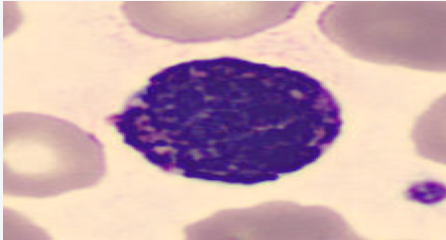
\includegraphics[width=0.95cm,height=0.52cm,keepaspectratio]{figures/sample_blood.png}}} \\
\rowcolor{gray!10}
Derma & 7 & 7,007 & 1,003 & 2,005 & 10,015 & \makebox[1.05cm][c]{\raisebox{-0.16cm}{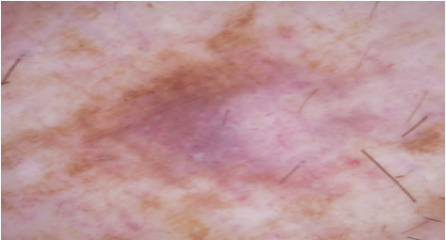
\includegraphics[width=0.95cm,height=0.52cm,keepaspectratio]{figures/sample_derma.png}}} \\
Organ-C & 11 & 12,975 & 2,392 & 8,216 & 23,583 & \makebox[1.05cm][c]{\raisebox{-0.16cm}{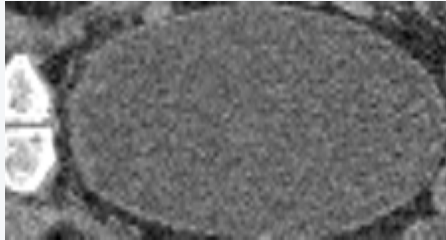
\includegraphics[width=0.95cm,height=0.52cm,keepaspectratio]{figures/sample_organ_c.png}}} \\
\rowcolor{gray!10}
Organ-S & 11 & 13,932 & 2,452 & 8,827 & 25,211 & \makebox[1.05cm][c]{\raisebox{-0.16cm}{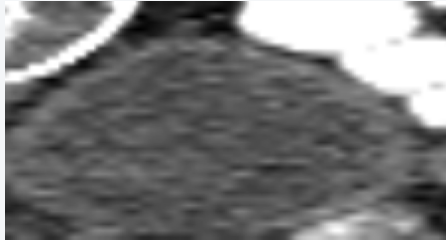
\includegraphics[width=0.95cm,height=0.52cm,keepaspectratio]{figures/sample_organ_s.png}}} \\
Ultrasound & 8 & 3,869 & 549 & 1,113 & 5,531 & \makebox[1.05cm][c]{\raisebox{-0.16cm}{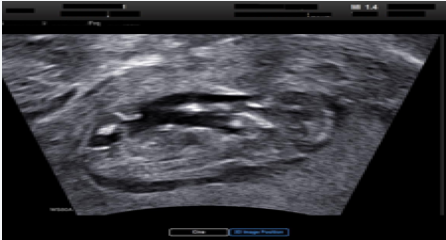
\includegraphics[width=0.95cm,height=0.52cm,keepaspectratio]{figures/sample_ultrasound.png}}} \\
\noalign{\hrule height 1.25pt}
\end{tabular}
}
\end{table}

\subsubsection{(2) Baselines:}

We compare LAMP-Merge with twelve established merging baselines spanning parameter averaging, task-vector pruning, conflict resolution, statistic-aware correction, interpolation, subspace merging, Fourier fusion, and robust merging~\cite{yadav2023tiesmergingresolvinginterferencemerging,yu2024languagemodelssupermario,jin2025datalessknowledgefusionmerging,wu_parameter_2025,davari2024modelbreadcrumbsscalingmultitask,jang2025modelstockneedjust,ilharco2023editingmodelstaskarithmetic,marczak2025taskleftbehindisotropic,zheng2025freemergingfouriertransformefficient,zeng2025robustmergeparameterefficientmodelmerging}.

\subsubsection{(3) Merging Settings:}


% Experiments follow a single-shot asynchronous model-merging protocol. Each client independently trains a local model on its own medical imaging data and then computes the class-level statistics required by LAMP-Merge locally, including class-support counts, reference-space class prototypes, and class-prevalence counts. These statistics are uploaded once together with an interface to the local checkpoint. The server performs a single model-merging step using only the uploaded checkpoints and class-level statistics, and evaluates the resulting merged model on a global test set.

We evaluate four vision-model families: ResNet, ConvNeXt, ViT-Tiny, and Swin-Tiny\cite{he2016deep,liu2022convnet,dosovitskiy2021image,liu2021swin}. For each dataset-model pair, we construct non-IID client partitions with $K\in\{3,5,7\}$ clients and Dirichlet skew parameter $\beta\in\{0,0.01,0.1\}$, using seed 42\cite{hsu2019measuringeffectsnonidenticaldata}. A client-average result fixes the dataset, model, and $K$, and then averages over the three $\beta$ values. And the experiments follow a single-shot asynchronous model-merging protocol.

% \subsubsection{4) Implementation Environment:}

% All experiments were run on a server with two Intel(R) Xeon(R) Silver 4210 CPUs, four NVIDIA GeForce RTX 2080 Ti GPUs, and the conda environment \texttt{MM} with Python 3.10.20, PyTorch 2.6.0+\texttt{cu118}, and CUDA runtime 11.8.

\subsection{Comparison With the State of the Arts}

% The main comparison uses client-average ACC: for each fixed dataset, model, and client number, we first average over the three $\beta$ skew levels and then compare merging methods. A cell is counted as successful when LAMP-Merge is greater than or equal to the strongest non-LAMP baseline in that cell.

Tables~\ref{tab:client-avg-resnet}--\ref{tab:client-avg-swin-tiny} report the full client-average results for all four backbones. Across all evaluated settings, LAMP-Merge wins or ties the strongest non-LAMP baseline in \textbf{57 cells (95.0\%)}.

\setcounter{dbltopnumber}{4}
\setcounter{topnumber}{4}
\setcounter{totalnumber}{4}

\begin{table*}[!t]
\centering
\renewcommand{\arraystretch}{1.35}
\caption{Client-average test accuracy / Macro-F1 (\%) on ResNet. Each entry is reported as ACC / F1, where F1 denotes Macro-F1 and each value averages the three Dirichlet settings for a fixed client number; Avg averages $K=3,5,7$ within the corresponding dataset.}
\label{tab:client-avg-resnet}
\resizebox{\textwidth}{!}{%
\begin{tabular}{l||ccc:c|ccc:c|ccc:c|ccc:c|ccc:c}
\noalign{\hrule height 1.25pt}
\rowcolor[HTML]{F2F2F2}
 &
\multicolumn{4}{c|}{\textbf{Blood}} &
\multicolumn{4}{c|}{\textbf{Derma}} &
\multicolumn{4}{c|}{\textbf{Organ-C}} &
\multicolumn{4}{c|}{\textbf{Organ-S}} &
\multicolumn{4}{c}{\textbf{Ultrasound}} \\
\rowcolor[HTML]{F2F2F2}
\multirow{-2}{*}{\textbf{Method}}
& \textbf{$K=3$} & \textbf{$K=5$} & \textbf{$K=7$} & \textbf{Avg}
& \textbf{$K=3$} & \textbf{$K=5$} & \textbf{$K=7$} & \textbf{Avg}
& \textbf{$K=3$} & \textbf{$K=5$} & \textbf{$K=7$} & \textbf{Avg}
& \textbf{$K=3$} & \textbf{$K=5$} & \textbf{$K=7$} & \textbf{Avg}
& \textbf{$K=3$} & \textbf{$K=5$} & \textbf{$K=7$} & \textbf{Avg} \\
\hline \hline

Weight Avg. & 33.45 / 23.94 & 24.67 / 15.61 & 28.22 / 14.88 & 28.78 / 18.14 & 62.91 / 13.63 & 47.00 / 11.83 & 62.44 / 13.44 & 57.45 / 12.97 & 22.61 / 12.19 & 17.72 / 9.10 & 13.96 / 6.49 & 18.10 / 9.26 & 28.64 / 16.12 & 17.94 / 9.68 & 24.75 / 9.13 & 23.78 / 11.64 & 24.35 / 12.05 & 15.81 / 6.89 & 15.42 / 4.50 & 18.53 / 7.81 \\

\rowcolor{gray!10}
TIES\pub{NeurIPS 2023} & 26.01 / 15.52 & 18.72 / 6.45 & 17.87 / 6.48 & 20.87 / 9.48 & 59.95 / 17.19 & 48.41 / 9.06 & 64.84 / 12.59 & 57.73 / 12.95 & 26.50 / 14.04 & 16.84 / 10.62 & 21.18 / 9.84 & 21.51 / 11.50 & 19.81 / 10.76 & 19.15 / 10.56 & 18.74 / 6.21 & 19.23 / 9.18 & 34.77 / 25.99 & 19.89 / 11.44 & 18.54 / 7.58 & 24.40 / 15.00 \\

DARE-Linear\pub{ICML 2024} & 28.32 / 18.65 & 28.56 / 15.87 & 23.92 / 10.84 & 26.93 / 15.12 & 63.57 / 14.49 & 48.41 / 11.06 & 62.88 / 13.03 & 58.29 / 12.86 & 20.18 / 8.37 & 25.88 / 10.20 & 16.50 / 6.84 & 20.85 / 8.47 & 25.45 / 11.52 & 22.45 / 9.05 & 25.37 / 8.26 & 24.42 / 9.61 & 21.62 / 9.40 & 17.28 / 8.28 & 16.08 / 4.93 & 18.33 / 7.53 \\

\rowcolor{gray!10}
DARE-TIES\pub{ICML 2024} & 31.94 / 19.01 & 19.35 / 6.63 & 17.80 / 7.03 & 23.03 / 10.89 & 53.75 / 11.16 & 48.25 / 8.70 & 55.58 / 10.94 & 52.53 / 10.27 & 18.51 / 7.52 & 15.15 / 7.22 & 18.59 / 7.54 & 17.42 / 7.43 & 17.90 / 10.39 & 13.52 / 6.84 & 17.30 / 7.61 & 16.24 / 8.28 & 29.32 / 20.58 & 16.35 / 8.63 & 18.90 / 7.67 & 21.52 / 12.29 \\

RegMean\pub{ICLR 2023} & 34.60 / 25.73 & 23.69 / 17.43 & 34.07 / 19.68 & 30.79 / 20.95 & 58.12 / 16.28 & 28.43 / 14.49 & 50.22 / 15.32 & 45.59 / 15.36 & 24.05 / 15.91 & 13.40 / 11.81 & 13.88 / 7.91 & 17.11 / 11.88 & 25.04 / 16.75 & 16.23 / 12.52 & 14.93 / 7.07 & 18.73 / 12.11 & 22.76 / 17.86 & 16.95 / 15.76 & 13.18 / 15.47 & 17.63 / 16.36 \\

\rowcolor{gray!10}
Fisher\pub{NeurIPS 2022} & 31.96 / 26.20 & 22.37 / 13.84 & 26.08 / 6.73 & 26.80 / 15.59 & 67.07 / 16.51 & 67.02 / 12.67 & 66.90 / 11.54 & 67.00 / 13.58 & 29.73 / 22.82 & 17.41 / 23.98 & 18.12 / 11.32 & 21.75 / 19.37 & 20.10 / 16.73 & 29.56 / 17.28 & 19.63 / 9.70 & 23.10 / 14.57 & 23.33 / 18.98 & 18.60 / 18.22 & 25.13 / 11.18 & 22.35 / 16.13 \\

Breadcrumbs\pub{ECCV 2024} & 8.54 / 3.18 & 14.17 / 5.35 & 14.60 / 6.13 & 12.44 / 4.89 & 4.95 / 1.94 & 29.13 / 7.30 & 17.21 / 5.39 & 17.10 / 4.88 & 7.66 / 1.79 & 6.76 / 2.68 & 6.85 / 2.60 & 7.09 / 2.36 & 8.02 / 2.73 & 9.48 / 3.68 & 6.03 / 1.91 & 7.84 / 2.77 & 12.25 / 3.32 & 12.73 / 5.09 & 10.21 / 5.50 & 11.73 / 4.64 \\

\rowcolor{gray!10}
Model Stock\pub{ECCV 2024} & 24.20 / 16.77 & 18.24 / 8.12 & 19.75 / 6.48 & 20.73 / 10.45 & 62.16 / 14.60 & 43.11 / 10.80 & 57.21 / 13.08 & 54.16 / 12.83 & 12.25 / 3.93 & 12.74 / 6.03 & 11.85 / 3.01 & 12.28 / 4.32 & 27.42 / 14.71 & 15.78 / 7.86 & 20.12 / 5.99 & 21.11 / 9.52 & 17.91 / 8.10 & 13.21 / 5.94 & 15.78 / 4.44 & 15.63 / 6.16 \\

Iso-C\pub{ICML 2025} & 32.78 / 23.32 & 27.48 / 17.39 & 30.23 / 15.01 & 30.16 / 18.57 & 50.49 / 15.02 & 44.22 / 16.17 & 64.16 / 14.32 & 52.96 / 15.17 & 23.31 / 12.98 & 16.29 / 7.96 & 13.83 / 6.14 & 17.81 / 9.03 & 27.36 / 14.97 & 21.18 / 11.80 & 24.53 / 8.07 & 24.36 / 11.61 & 26.15 / 15.77 & 16.98 / 8.93 & 15.54 / 5.75 & 19.56 / 10.15 \\

\rowcolor{gray!10}
Free-Merging\pub{ICCV 2025} & 33.45 / 23.95 & 24.67 / 15.63 & 28.22 / 14.89 & 28.78 / 18.16 & 62.91 / 13.62 & 47.00 / 11.83 & 62.46 / 13.45 & 57.46 / 12.97 & 22.61 / 12.19 & 17.71 / 9.10 & 13.96 / 6.49 & 18.09 / 9.26 & 28.63 / 16.12 & 17.93 / 9.68 & 24.75 / 9.12 & 23.77 / 11.64 & 24.35 / 12.05 & 15.81 / 6.88 & 15.45 / 4.51 & 18.54 / 7.81 \\

RobustMerge\pub{NeurIPS 2025} & 34.01 / 20.06 & 24.30 / 13.12 & 22.56 / 9.35 & 26.96 / 14.18 & 29.56 / 11.45 & 20.85 / 9.33 & 39.42 / 14.11 & 29.94 / 11.63 & 24.58 / 13.59 & 17.64 / 9.42 & 16.53 / 6.77 & 19.58 / 9.93 & 26.80 / 12.52 & 22.27 / 13.00 & 23.01 / 9.31 & 24.03 / 11.61 & 21.89 / 11.26 & 22.31 / 12.73 & 17.07 / 7.26 & 20.42 / 10.42 \\

\rowcolor{gray!10}
FROM\pub{AAAI 2026} & 29.89 / 18.76 & 23.06 / 11.03 & 20.52 / 8.00 & 24.49 / 12.60 & 67.13 / 13.11 & 43.69 / 10.22 & 65.80 / 12.95 & 58.87 / 12.09 & 23.50 / 13.76 & 15.60 / 9.50 & 15.20 / 5.57 & 18.10 / 9.61 & 22.07 / 12.49 & 20.87 / 11.30 & 24.76 / 8.15 & 22.57 / 10.64 & 23.09 / 11.06 & 15.06 / 7.44 & 20.63 / 8.82 & 19.59 / 9.11 \\

\hline \hline
\rowcolor[HTML]{FFF9C4}
\textbf{LAMP-Merge} & \tworowbestreshl{\textbf{80.01 / 78.72}}{45.41} & \tworowbestreshl{\textbf{79.94 / 78.67}}{51.38} & \tworowbestreshl{\textbf{79.92 / 78.65}}{45.85} & \tworowbestreshl{\textbf{79.95 / 78.68}}{49.16} & \tworowbestreshl{\textbf{67.55 / 15.03}}{0.42} & \tworowbestreshl{\textbf{67.63 / 15.16}}{0.61} & \tworowbestreshl{\textbf{67.63 / 14.94}}{0.73} & \tworowbestreshl{\textbf{67.60 / 15.04}}{0.60} & \tworowbestreshl{\textbf{60.05 / 53.15}}{30.32} & \tworowbestreshl{\textbf{59.94 / 52.98}}{34.06} & \tworowbestreshl{\textbf{60.07 / 53.28}}{38.89} & \tworowbestreshl{\textbf{60.02 / 53.14}}{38.27} & \tworowbestreshl{\textbf{52.98 / 42.85}}{24.34} & \tworowbestreshl{\textbf{52.79 / 42.54}}{23.23} & \tworowbestreshl{\textbf{52.81 / 42.31}}{27.44} & \tworowbestreshl{\textbf{52.86 / 42.57}}{28.44} & \tworowbestreshl{\textbf{48.07 / 45.96}}{13.30} & \tworowbestreshl{\textbf{46.75 / 44.46}}{24.44} & \tworowbestreshl{\textbf{47.35 / 45.08}}{22.22} & \tworowbestreshl{\textbf{47.39 / 45.17}}{22.99} \\
\noalign{\hrule height 1.25pt}
\end{tabular}%
}
\end{table*}

\begin{table*}[!t]
\centering
\renewcommand{\arraystretch}{1.35}
\caption{Client-average test accuracy / Macro-F1 (\%) on ConvNeXt. Each entry is reported as ACC / F1, where F1 denotes Macro-F1 and each value averages the three Dirichlet settings for a fixed client number; Avg averages $K=3,5,7$ within the corresponding dataset.}
\label{tab:client-avg-convnext}
\resizebox{\textwidth}{!}{%
\begin{tabular}{l||ccc:c|ccc:c|ccc:c|ccc:c|ccc:c}
\noalign{\hrule height 1.25pt}
\rowcolor[HTML]{F2F2F2}
 &
\multicolumn{4}{c|}{\textbf{Blood}} &
\multicolumn{4}{c|}{\textbf{Derma}} &
\multicolumn{4}{c|}{\textbf{Organ-C}} &
\multicolumn{4}{c|}{\textbf{Organ-S}} &
\multicolumn{4}{c}{\textbf{Ultrasound}} \\
\rowcolor[HTML]{F2F2F2}
\multirow{-2}{*}{\textbf{Method}}
& \textbf{$K=3$} & \textbf{$K=5$} & \textbf{$K=7$} & \textbf{Avg}
& \textbf{$K=3$} & \textbf{$K=5$} & \textbf{$K=7$} & \textbf{Avg}
& \textbf{$K=3$} & \textbf{$K=5$} & \textbf{$K=7$} & \textbf{Avg}
& \textbf{$K=3$} & \textbf{$K=5$} & \textbf{$K=7$} & \textbf{Avg}
& \textbf{$K=3$} & \textbf{$K=5$} & \textbf{$K=7$} & \textbf{Avg} \\
\hline \hline

Weight Avg. & 15.65 / 3.37 & 11.22 / 2.48 & 13.84 / 3.00 & 13.57 / 2.95 & 29.66 / 5.71 & 48.30 / 8.59 & 66.88 / 11.45 & 48.28 / 8.58 & 10.37 / 2.79 & 12.18 / 1.91 & 9.44 / 1.57 & 10.66 / 2.09 & 13.08 / 2.04 & 10.35 / 1.69 & 14.16 / 2.20 & 12.53 / 1.98 & 15.06 / 3.26 & 15.06 / 3.26 & 12.52 / 2.77 & 14.21 / 3.09 \\

\rowcolor{gray!10}
TIES\pub{NeurIPS 2023} & 17.15 / 3.65 & 12.14 / 2.67 & 15.24 / 3.30 & 14.84 / 3.21 & 29.66 / 5.71 & 17.97 / 5.62 & 27.13 / 5.12 & 24.92 / 5.48 & 12.17 / 4.98 & 7.86 / 1.43 & 7.16 / 1.61 & 9.06 / 2.67 & 11.23 / 3.07 & 7.61 / 2.02 & 7.96 / 1.40 & 8.93 / 2.16 & 15.18 / 3.28 & 14.56 / 3.15 & 12.91 / 2.84 & 14.22 / 3.09 \\

DARE-Linear\pub{ICML 2024} & 17.56 / 3.76 & 11.22 / 2.48 & 13.45 / 2.92 & 14.08 / 3.05 & 27.05 / 5.06 & 48.30 / 8.59 & 48.30 / 8.59 & 41.22 / 7.41 & 10.35 / 2.40 & 6.99 / 1.18 & 10.85 / 1.78 & 9.40 / 1.79 & 12.82 / 2.16 & 10.35 / 1.69 & 7.97 / 1.33 & 10.38 / 1.73 & 15.75 / 3.39 & 15.75 / 3.39 & 12.64 / 2.79 & 14.71 / 3.19 \\

\rowcolor{gray!10}
DARE-TIES\pub{ICML 2024} & 10.96 / 3.30 & 15.19 / 3.27 & 14.97 / 3.66 & 13.71 / 3.41 & 9.08 / 2.36 & 27.98 / 7.91 & 24.51 / 4.47 & 20.52 / 4.91 & 13.05 / 4.57 & 13.46 / 3.30 & 7.70 / 1.47 & 11.40 / 3.11 & 10.96 / 3.43 & 9.46 / 2.64 & 7.09 / 1.58 & 9.17 / 2.55 & 14.56 / 3.15 & 12.97 / 2.85 & 15.00 / 3.26 & 14.18 / 3.09 \\

RegMean\pub{ICLR 2023} & 15.65 / 3.37 & 8.17 / 1.89 & 18.56 / 5.87 & 14.13 / 3.71 & 26.33 / 4.87 & 7.73 / 2.03 & 27.20 / 5.07 & 20.42 / 3.99 & 11.43 / 3.99 & 10.17 / 2.43 & 7.68 / 1.64 & 9.76 / 2.68 & 10.14 / 4.29 & 12.59 / 4.42 & 10.38 / 3.14 & 11.04 / 3.95 & 15.75 / 3.39 & 15.39 / 3.33 & 15.00 / 2.91 & 15.38 / 3.21 \\

\rowcolor{gray!10}
Fisher\pub{NeurIPS 2022} & 15.65 / 3.37 & 9.99 / 2.26 & 11.89 / 2.71 & 12.51 / 2.78 & 48.25 / 8.58 & 26.38 / 4.88 & 29.71 / 5.72 & 34.78 / 6.39 & 10.03 / 3.63 & 9.74 / 2.45 & 9.15 / 1.44 & 9.64 / 2.51 & 6.04 / 2.23 & 5.17 / 0.99 & 8.43 / 3.15 & 6.55 / 2.13 & 16.95 / 3.62 & 13.60 / 3.39 & 14.56 / 3.15 & 15.04 / 3.39 \\

Breadcrumbs\pub{ECCV 2024} & 15.16 / 3.26 & 13.66 / 2.97 & 11.63 / 2.55 & 13.48 / 2.93 & 5.24 / 1.38 & 27.66 / 5.22 & 46.30 / 8.10 & 26.40 / 4.90 & 10.31 / 1.70 & 14.44 / 2.35 & 15.74 / 3.09 & 13.50 / 2.38 & 15.16 / 2.35 & 15.54 / 2.40 & 20.77 / 3.11 & 17.16 / 2.62 & 13.84 / 3.03 & 13.63 / 2.99 & 13.63 / 2.99 & 13.70 / 3.00 \\

\rowcolor{gray!10}
Model Stock\pub{ECCV 2024} & 17.56 / 3.72 & 11.44 / 2.54 & 17.78 / 3.80 & 15.59 / 3.35 & 29.66 / 5.71 & 48.30 / 8.59 & 66.88 / 11.45 & 48.28 / 8.58 & 12.76 / 3.72 & 12.18 / 1.91 & 13.85 / 2.17 & 12.93 / 2.60 & 13.08 / 2.04 & 10.35 / 1.69 & 19.35 / 2.91 & 14.26 / 2.21 & 15.75 / 3.39 & 12.91 / 2.84 & 14.79 / 3.21 & 14.48 / 3.15 \\

Iso-C\pub{ICML 2025} & 19.47 / 4.07 & 18.65 / 3.93 & 14.80 / 3.22 & 17.64 / 3.74 & 29.71 / 5.72 & 48.30 / 8.59 & 66.88 / 11.45 & 48.30 / 8.59 & 9.91 / 2.18 & 6.99 / 1.18 & 9.45 / 1.65 & 8.78 / 1.67 & 7.89 / 1.33 & 14.77 / 2.28 & 8.67 / 3.00 & 10.44 / 2.20 & 15.18 / 3.28 & 12.91 / 2.84 & 16.05 / 3.50 & 14.71 / 3.21 \\

\rowcolor{gray!10}
Free-Merging\pub{ICCV 2025} & 15.75 / 3.35 & 11.90 / 2.61 & 13.84 / 3.00 & 13.83 / 2.99 & 29.71 / 5.72 & 48.30 / 8.59 & 66.88 / 11.45 & 48.30 / 8.59 & 9.06 / 1.55 & 12.18 / 1.91 & 13.85 / 2.17 & 11.70 / 1.87 & 13.08 / 2.04 & 10.35 / 1.69 & 14.16 / 2.20 & 12.53 / 1.98 & 15.06 / 3.26 & 12.91 / 2.84 & 16.95 / 3.92 & 14.97 / 3.34 \\

RobustMerge\pub{NeurIPS 2025} & 14.10 / 3.06 & 14.05 / 3.05 & 7.52 / 1.75 & 11.89 / 2.62 & 9.08 / 2.36 & 45.07 / 7.77 & 48.30 / 8.59 & 34.15 / 6.24 & 13.94 / 2.34 & 12.18 / 1.91 & 17.93 / 2.72 & 14.68 / 2.32 & 23.54 / 3.47 & 9.61 / 1.57 & 20.77 / 3.11 & 17.97 / 2.72 & 13.00 / 2.86 & 11.35 / 2.55 & 13.63 / 2.99 & 12.66 / 2.80 \\

\rowcolor{gray!10}
FROM\pub{AAAI 2026} & 15.65 / 3.37 & 10.83 / 2.39 & 16.71 / 3.57 & 14.40 / 3.11 & 29.66 / 5.71 & 34.06 / 8.52 & 45.69 / 7.94 & 36.47 / 7.39 & 12.32 / 3.83 & 12.24 / 1.92 & 6.50 / 1.10 & 10.35 / 2.28 & 13.24 / 3.47 & 11.05 / 2.64 & 8.97 / 1.49 & 11.09 / 2.54 & 15.75 / 3.39 & 15.78 / 3.40 & 10.87 / 2.45 & 14.13 / 3.08 \\

\hline \hline
\rowcolor[HTML]{FFF9C4}
\textbf{LAMP-Merge} & \tworowbestreshl{\textbf{84.85 / 83.43}}{65.38} & \tworowbestreshl{\textbf{84.87 / 83.47}}{66.22} & \tworowbestreshl{\textbf{84.98 / 83.54}}{66.42} & \tworowbestreshl{\textbf{84.90 / 83.48}}{67.26} & \tworowbestreshl{\textbf{59.68 / 33.64}}{11.43} & \tworowbestreshl{\textbf{58.77 / 32.92}}{10.47} & \tworowbestreshl{\textbf{59.42 / 33.42}}{7.46} & \tworowbestreshl{\textbf{59.29 / 33.33}}{10.99} & \tworowbestreshl{\textbf{65.41 / 63.17}}{51.47} & \tworowbestreshl{\textbf{65.33 / 63.11}}{50.89} & \tworowbestreshl{\textbf{65.51 / 63.23}}{47.58} & \tworowbestreshl{\textbf{65.42 / 63.17}}{50.74} & \tworowbestreshl{\textbf{60.55 / 56.03}}{37.01} & \tworowbestreshl{\textbf{60.50 / 56.04}}{44.96} & \tworowbestreshl{\textbf{60.66 / 56.04}}{39.89} & \tworowbestreshl{\textbf{60.57 / 56.04}}{42.60} & \tworowbestreshl{\textbf{43.07 / 41.00}}{26.12} & \tworowbestreshl{\textbf{42.80 / 40.79}}{27.02} & \tworowbestreshl{\textbf{42.41 / 40.36}}{25.46} & \tworowbestreshl{\textbf{42.76 / 40.72}}{27.38} \\
\end{tabular}%
}
\end{table*}

\begin{table*}[!t]
\centering
\renewcommand{\arraystretch}{1.35}
\caption{Client-average test accuracy / Macro-F1 (\%) on ViT-Tiny. Each entry is reported as ACC / F1, where F1 denotes Macro-F1 and each value averages the three Dirichlet settings for a fixed client number; Avg averages $K=3,5,7$ within the corresponding dataset.}
\label{tab:client-avg-vit-t}
\resizebox{\textwidth}{!}{%
\begin{tabular}{l||ccc:c|ccc:c|ccc:c|ccc:c|ccc:c}
\noalign{\hrule height 1.25pt}
\rowcolor[HTML]{F2F2F2}
 &
\multicolumn{4}{c|}{\textbf{Blood}} &
\multicolumn{4}{c|}{\textbf{Derma}} &
\multicolumn{4}{c|}{\textbf{Organ-C}} &
\multicolumn{4}{c|}{\textbf{Organ-S}} &
\multicolumn{4}{c}{\textbf{Ultrasound}} \\
\rowcolor[HTML]{F2F2F2}
\multirow{-2}{*}{\textbf{Method}}
& \textbf{$K=3$} & \textbf{$K=5$} & \textbf{$K=7$} & \textbf{Avg}
& \textbf{$K=3$} & \textbf{$K=5$} & \textbf{$K=7$} & \textbf{Avg}
& \textbf{$K=3$} & \textbf{$K=5$} & \textbf{$K=7$} & \textbf{Avg}
& \textbf{$K=3$} & \textbf{$K=5$} & \textbf{$K=7$} & \textbf{Avg}
& \textbf{$K=3$} & \textbf{$K=5$} & \textbf{$K=7$} & \textbf{Avg} \\
\hline \hline

Weight Avg. & 13.43 / 4.05 & 10.82 / 2.39 & 11.60 / 3.15 & 11.95 / 3.19 & 46.38 / 8.14 & 43.69 / 11.46 & 36.96 / 8.44 & 42.34 / 9.35 & 16.57 / 7.59 & 10.43 / 3.88 & 9.52 / 4.01 & 12.17 / 5.16 & 8.44 / 3.70 & 8.52 / 2.91 & 17.10 / 5.24 & 11.35 / 3.95 & 14.50 / 3.58 & 13.27 / 3.56 & 18.84 / 7.56 & 15.54 / 4.90 \\

\rowcolor{gray!10}
TIES\pub{NeurIPS 2023} & 7.96 / 3.42 & 14.21 / 5.13 & 12.85 / 3.43 & 11.67 / 3.99 & 47.80 / 9.19 & 34.98 / 8.17 & 46.15 / 8.46 & 42.98 / 8.61 & 13.41 / 6.55 & 12.23 / 4.69 & 9.53 / 3.40 & 11.72 / 4.88 & 11.92 / 3.97 & 10.02 / 2.66 & 15.97 / 5.94 & 12.64 / 4.19 & 20.01 / 9.29 & 13.06 / 4.93 & 10.18 / 2.58 & 14.42 / 5.60 \\

DARE-Linear\pub{ICML 2024} & 23.97 / 12.03 & 11.29 / 3.46 & 13.87 / 4.27 & 16.38 / 6.59 & 28.50 / 5.74 & 10.02 / 3.26 & 12.04 / 5.72 & 16.85 / 4.91 & 15.34 / 8.12 & 9.46 / 2.88 & 7.04 / 2.83 & 10.61 / 4.61 & 7.48 / 3.58 & 5.49 / 1.28 & 16.11 / 5.28 & 9.69 / 3.38 & 13.66 / 3.89 & 10.51 / 2.38 & 14.35 / 3.21 & 12.84 / 3.16 \\

\rowcolor{gray!10}
DARE-TIES\pub{ICML 2024} & 7.35 / 2.90 & 11.89 / 2.61 & 11.46 / 2.81 & 10.23 / 2.77 & 27.35 / 6.66 & 45.02 / 9.40 & 35.28 / 8.36 & 35.88 / 8.14 & 12.52 / 5.80 & 9.03 / 4.08 & 10.33 / 3.58 & 10.63 / 4.49 & 5.41 / 1.64 & 8.74 / 2.73 & 5.91 / 2.50 & 6.69 / 2.29 & 14.47 / 5.16 & 11.20 / 3.72 & 10.42 / 3.00 & 12.03 / 3.96 \\

RegMean\pub{ICLR 2023} & 17.48 / 8.00 & 14.17 / 6.17 & 12.90 / 2.95 & 14.85 / 5.71 & 51.14 / 10.12 & 36.67 / 8.86 & 66.58 / 11.44 & 51.46 / 10.14 & 12.50 / 4.50 & 9.64 / 3.44 & 9.83 / 4.00 & 10.66 / 3.98 & 12.63 / 5.96 & 7.17 / 2.21 & 10.68 / 2.68 & 10.16 / 3.62 & 14.91 / 5.37 & 13.84 / 6.75 & 11.44 / 6.60 & 13.40 / 6.24 \\

\rowcolor{gray!10}
Fisher\pub{NeurIPS 2022} & 11.66 / 2.74 & 15.12 / 3.09 & 19.44 / 7.18 & 15.41 / 4.34 & 47.80 / 8.99 & 20.42 / 7.27 & 48.20 / 9.57 & 38.81 / 8.61 & 7.99 / 5.93 & 10.72 / 3.80 & 14.24 / 3.58 & 10.98 / 4.44 & 8.56 / 4.06 & 12.18 / 4.07 & 12.22 / 5.92 & 10.99 / 4.68 & 16.11 / 9.45 & 13.15 / 5.22 & 14.20 / 3.20 & 14.49 / 5.96 \\

Breadcrumbs\pub{ECCV 2024} & 13.63 / 3.67 & 10.39 / 2.34 & 13.00 / 3.72 & 12.34 / 3.24 & 4.89 / 1.99 & 25.72 / 4.75 & 6.07 / 3.14 & 12.23 / 3.29 & 7.73 / 2.44 & 10.00 / 5.62 & 16.44 / 4.60 & 11.39 / 4.22 & 12.37 / 4.42 & 4.83 / 1.76 & 12.19 / 3.51 & 9.80 / 3.23 & 13.60 / 4.96 & 11.41 / 2.71 & 15.24 / 3.87 & 13.42 / 3.85 \\

\rowcolor{gray!10}
Model Stock\pub{ECCV 2024} & 19.40 / 6.62 & 11.20 / 3.74 & 11.34 / 3.14 & 13.98 / 4.50 & 38.05 / 7.67 & 30.79 / 7.56 & 27.35 / 7.04 & 32.06 / 7.42 & 14.88 / 7.82 & 12.27 / 6.18 & 12.15 / 4.29 & 13.10 / 6.10 & 8.93 / 3.35 & 8.59 / 3.27 & 18.67 / 6.91 & 12.06 / 4.51 & 15.99 / 5.30 & 18.09 / 6.89 & 16.41 / 4.46 & 16.83 / 5.55 \\

Iso-C\pub{ICML 2025} & 12.34 / 3.63 & 14.83 / 5.69 & 10.18 / 3.41 & 12.45 / 4.24 & 57.09 / 11.23 & 45.29 / 11.31 & 23.06 / 7.63 & 41.81 / 10.06 & 10.84 / 4.97 & 5.67 / 1.78 & 8.97 / 5.53 & 8.49 / 4.09 & 6.11 / 2.27 & 5.31 / 2.29 & 10.81 / 5.45 & 7.41 / 3.34 & 14.17 / 5.75 & 15.27 / 6.49 & 18.69 / 8.56 & 16.04 / 6.93 \\

\rowcolor{gray!10}
Free-Merging\pub{ICCV 2025} & 19.89 / 7.03 & 14.57 / 6.11 & 13.92 / 5.51 & 16.13 / 6.22 & 46.30 / 8.10 & 47.70 / 9.56 & 38.55 / 9.31 & 44.18 / 8.99 & 14.25 / 5.22 & 9.80 / 4.05 & 7.59 / 3.26 & 10.55 / 4.18 & 7.27 / 2.91 & 9.14 / 3.42 & 16.43 / 4.71 & 10.95 / 3.68 & 14.05 / 3.22 & 15.93 / 4.71 & 16.47 / 6.19 & 15.48 / 4.71 \\

RobustMerge\pub{NeurIPS 2025} & 14.82 / 3.29 & 10.70 / 3.15 & 14.25 / 3.47 & 13.26 / 3.30 & 3.47 / 1.10 & 27.68 / 5.27 & 17.24 / 8.45 & 16.13 / 4.94 & 9.54 / 3.90 & 6.17 / 2.08 & 14.38 / 5.33 & 10.03 / 3.77 & 12.60 / 3.27 & 7.07 / 4.07 & 12.17 / 2.61 & 10.61 / 3.32 & 16.98 / 6.77 & 18.54 / 7.33 & 15.63 / 4.37 & 17.05 / 6.16 \\

\rowcolor{gray!10}
FROM\pub{AAAI 2026} & 18.02 / 8.54 & 7.81 / 2.36 & 14.05 / 3.05 & 13.29 / 4.65 & 46.95 / 9.16 & 51.21 / 10.76 & 66.88 / 11.45 & 55.01 / 10.46 & 21.48 / 10.56 & 13.01 / 5.13 & 9.72 / 3.53 & 14.74 / 6.41 & 7.72 / 3.10 & 7.98 / 2.50 & 14.85 / 6.23 & 10.18 / 3.94 & 18.36 / 7.49 & 17.43 / 7.51 & 17.76 / 8.40 & 17.85 / 7.80 \\

\hline \hline
\rowcolor[HTML]{FFF9C4}
\textbf{LAMP-Merge} & \tworowbestreshl{\textbf{85.21 / 83.06}}{61.24} & \tworowbestreshl{\textbf{85.06 / 82.96}}{69.94} & \tworowbestreshl{\textbf{84.98 / 82.85}}{65.54} & \tworowbestreshl{\textbf{85.09 / 82.95}}{68.71} & \tworowbestreshl{\textbf{59.45 / 36.65}}{2.36} & \tworowbestreshl{\textbf{59.32 / 36.61}}{8.11} & \tworowbestreshl{\textbf{59.83 / 36.79}}{7.05} & \tworowbestreshl{\textbf{59.53 / 36.68}}{4.52} & \tworowbestreshl{\textbf{58.78 / 57.39}}{37.30} & \tworowbestreshl{\textbf{58.40 / 56.93}}{45.39} & \tworowbestreshl{\textbf{58.29 / 56.80}}{41.85} & \tworowbestreshl{\textbf{58.49 / 57.04}}{43.75} & \tworowbestreshl{\textbf{54.39 / 52.06}}{41.76} & \tworowbestreshl{\textbf{54.51 / 52.22}}{42.33} & \tworowbestreshl{\textbf{54.65 / 52.28}}{35.98} & \tworowbestreshl{\textbf{54.52 / 52.18}}{41.88} & \tworowbestreshl{\textbf{46.12 / 42.27}}{26.11} & \tworowbestreshl{\textbf{45.97 / 42.23}}{27.43} & \tworowbestreshl{\textbf{45.94 / 42.15}}{27.10} & \tworowbestreshl{\textbf{46.01 / 42.22}}{28.16} \\
\end{tabular}%
}
\end{table*}

\begin{table*}[!t]
\centering
\renewcommand{\arraystretch}{1.35}
\caption{Client-average test accuracy / Macro-F1 (\%) on Swin-Tiny. Each entry is reported as ACC / F1, where F1 denotes Macro-F1 and each value averages the three Dirichlet settings for a fixed client number; Avg averages $K=3,5,7$ within the corresponding dataset.}
\label{tab:client-avg-swin-tiny}
\resizebox{\textwidth}{!}{%
\begin{tabular}{l||ccc:c|ccc:c|ccc:c|ccc:c|ccc:c}
\noalign{\hrule height 1.25pt}
\rowcolor[HTML]{F2F2F2}
 &
\multicolumn{4}{c|}{\textbf{Blood}} &
\multicolumn{4}{c|}{\textbf{Derma}} &
\multicolumn{4}{c|}{\textbf{Organ-C}} &
\multicolumn{4}{c|}{\textbf{Organ-S}} &
\multicolumn{4}{c}{\textbf{Ultrasound}} \\
\rowcolor[HTML]{F2F2F2}
\multirow{-2}{*}{\textbf{Method}}
& \textbf{$K=3$} & \textbf{$K=5$} & \textbf{$K=7$} & \textbf{Avg}
& \textbf{$K=3$} & \textbf{$K=5$} & \textbf{$K=7$} & \textbf{Avg}
& \textbf{$K=3$} & \textbf{$K=5$} & \textbf{$K=7$} & \textbf{Avg}
& \textbf{$K=3$} & \textbf{$K=5$} & \textbf{$K=7$} & \textbf{Avg}
& \textbf{$K=3$} & \textbf{$K=5$} & \textbf{$K=7$} & \textbf{Avg} \\
\hline \hline

Weight Avg. & 15.65 / 3.37 & 11.86 / 2.72 & 15.24 / 3.44 & 14.25 / 3.18 & 45.69 / 7.94 & 48.30 / 8.59 & 66.88 / 11.45 & 53.62 / 9.33 & 10.68 / 3.45 & 12.94 / 2.45 & 7.87 / 1.53 & 10.50 / 2.48 & 6.82 / 1.45 & 6.04 / 1.51 & 13.81 / 2.31 & 8.89 / 1.76 & 15.27 / 3.42 & 12.94 / 2.89 & 14.65 / 3.23 & 14.29 / 3.18 \\

\rowcolor{gray!10}
TIES\pub{NeurIPS 2023} & 9.72 / 2.20 & 11.90 / 2.61 & 13.84 / 3.00 & 11.82 / 2.60 & 8.41 / 2.19 & 7.80 / 2.01 & 66.88 / 11.45 & 27.70 / 5.22 & 11.60 / 3.92 & 7.02 / 1.40 & 9.34 / 1.92 & 9.32 / 2.41 & 7.34 / 2.39 & 6.07 / 1.10 & 11.07 / 2.28 & 8.16 / 1.92 & 16.95 / 5.90 & 13.03 / 2.98 & 12.61 / 3.51 & 14.20 / 4.13 \\

DARE-Linear\pub{ICML 2024} & 15.65 / 3.37 & 11.61 / 2.94 & 18.25 / 5.30 & 15.17 / 3.87 & 45.69 / 7.94 & 27.71 / 5.24 & 46.30 / 8.10 & 39.90 / 7.09 & 11.55 / 4.05 & 12.72 / 1.99 & 7.76 / 1.39 & 10.68 / 2.48 & 6.40 / 1.29 & 7.20 / 1.92 & 13.81 / 2.79 & 9.14 / 2.00 & 17.43 / 3.83 & 15.36 / 5.44 & 14.97 / 3.39 & 15.92 / 4.22 \\

\rowcolor{gray!10}
DARE-TIES\pub{ICML 2024} & 13.84 / 3.00 & 11.62 / 2.55 & 13.84 / 3.00 & 13.10 / 2.85 & 29.61 / 5.70 & 26.38 / 4.88 & 66.88 / 11.45 & 40.96 / 7.34 & 12.76 / 4.00 & 7.74 / 1.30 & 11.16 / 2.82 & 10.55 / 2.71 & 11.94 / 5.42 & 4.34 / 0.79 & 12.30 / 2.82 & 9.53 / 3.01 & 17.91 / 4.84 & 13.51 / 3.14 & 13.00 / 3.02 & 14.81 / 3.66 \\

RegMean\pub{ICLR 2023} & 13.74 / 3.02 & 17.15 / 3.65 & 15.78 / 3.43 & 15.56 / 3.37 & 27.05 / 5.06 & 46.30 / 8.10 & 45.69 / 7.94 & 39.68 / 7.03 & 14.11 / 6.71 & 7.73 / 1.30 & 8.11 / 1.36 & 9.98 / 3.12 & 12.15 / 3.40 & 8.21 / 1.58 & 9.26 / 1.90 & 9.87 / 2.29 & 14.65 / 6.19 & 11.05 / 4.14 & 17.79 / 8.55 & 14.50 / 6.29 \\

\rowcolor{gray!10}
Fisher\pub{NeurIPS 2022} & 16.33 / 3.37 & 17.56 / 3.72 & 15.65 / 3.37 & 16.51 / 3.49 & 45.82 / 11.46 & 6.52 / 1.72 & 47.18 / 8.23 & 33.17 / 7.14 & 8.14 / 3.23 & 8.99 / 1.49 & 9.78 / 3.19 & 8.97 / 2.64 & 6.51 / 1.82 & 6.50 / 2.40 & 10.92 / 4.10 & 7.98 / 2.77 & 17.46 / 6.16 & 11.65 / 3.60 & 17.55 / 4.13 & 15.55 / 4.63 \\

Breadcrumbs\pub{ECCV 2024} & 15.00 / 3.57 & 13.65 / 2.97 & 15.37 / 3.92 & 14.67 / 3.48 & 6.47 / 1.71 & 27.71 / 5.24 & 7.15 / 3.83 & 13.78 / 3.59 & 14.45 / 5.14 & 17.83 / 2.81 & 16.60 / 2.51 & 16.29 / 3.49 & 23.54 / 3.46 & 20.77 / 3.11 & 21.11 / 3.57 & 21.81 / 3.38 & 14.50 / 5.23 & 13.12 / 2.89 & 16.53 / 4.71 & 14.72 / 4.28 \\

\rowcolor{gray!10}
Model Stock\pub{ECCV 2024} & 13.74 / 3.02 & 14.40 / 3.55 & 17.15 / 3.65 & 15.10 / 3.41 & 45.69 / 7.94 & 27.71 / 5.24 & 48.25 / 8.79 & 40.55 / 7.32 & 11.10 / 3.38 & 7.71 / 1.49 & 14.04 / 2.91 & 10.95 / 2.59 & 6.71 / 1.43 & 11.06 / 3.00 & 17.14 / 4.69 & 11.64 / 3.04 & 15.39 / 3.60 & 12.73 / 3.24 & 18.69 / 7.22 & 15.60 / 4.69 \\

Iso-C\pub{ICML 2025} & 14.30 / 6.44 & 17.22 / 7.05 & 17.00 / 9.99 & 16.17 / 7.83 & 30.99 / 6.61 & 28.40 / 8.12 & 51.74 / 11.15 & 37.04 / 8.63 & 13.02 / 7.20 & 13.27 / 5.57 & 14.69 / 7.16 & 13.66 / 6.64 & 15.45 / 7.27 & 17.27 / 7.50 & 18.80 / 9.90 & 17.17 / 8.22 & 17.55 / 7.09 & 17.31 / 8.58 & 17.91 / 7.02 & 17.59 / 7.56 \\

\rowcolor{gray!10}
Free-Merging\pub{ICCV 2025} & 11.54 / 2.57 & 8.61 / 2.54 & 18.40 / 6.97 & 12.85 / 4.03 & 45.69 / 7.94 & 48.30 / 8.59 & 66.88 / 11.45 & 53.62 / 9.33 & 9.59 / 2.25 & 13.77 / 3.37 & 8.90 / 2.00 & 10.75 / 2.54 & 6.82 / 1.42 & 4.97 / 0.86 & 10.62 / 1.73 & 7.47 / 1.34 & 15.18 / 3.28 & 15.75 / 5.69 & 15.99 / 5.13 & 15.64 / 4.70 \\

RobustMerge\pub{NeurIPS 2025} & 13.74 / 3.02 & 14.09 / 3.14 & 16.70 / 3.60 & 14.84 / 3.26 & 23.77 / 4.23 & 27.71 / 5.24 & 5.04 / 1.46 & 18.84 / 3.64 & 16.01 / 4.91 & 14.42 / 2.35 & 19.60 / 3.97 & 16.68 / 3.74 & 16.73 / 4.92 & 11.51 / 3.64 & 20.77 / 3.11 & 16.34 / 3.89 & 17.61 / 6.32 & 13.15 / 3.03 & 16.29 / 5.38 & 15.68 / 4.91 \\

\rowcolor{gray!10}
FROM\pub{AAAI 2026} & 15.65 / 3.37 & 14.95 / 3.20 & 16.71 / 3.57 & 15.77 / 3.38 & 45.69 / 7.94 & 29.71 / 5.72 & 66.88 / 11.45 & 47.43 / 8.37 & 11.74 / 3.84 & 12.20 / 1.91 & 10.51 / 2.83 & 11.48 / 2.86 & 11.33 / 4.25 & 10.16 / 3.16 & 13.80 / 2.20 & 11.76 / 3.20 & 15.39 / 3.79 & 12.52 / 2.77 & 14.76 / 5.38 & 14.22 / 3.98 \\

\hline \hline
\rowcolor[HTML]{FFF9C4}
\textbf{LAMP-Merge} & \tworowbestreshl{\textbf{77.38 / 75.93}}{61.05} & \tworowbestreshl{\textbf{77.34 / 75.77}}{59.78} & \tworowbestreshl{\textbf{77.17 / 75.61}}{58.77} & \tworowbestreshl{\textbf{77.30 / 75.77}}{60.79} & \tworowbestreshl{\textbf{63.24 / 28.08}}{17.42} & \tworowbestreshl{\textbf{63.18 / 28.23}}{14.88} & \tworowbestreshl{\textbf{63.09 / 27.54}}{3.79} & \tworowbestreshl{\textbf{63.17 / 27.95}}{9.55} & \tworowbestreshl{\textbf{68.49 / 65.83}}{52.48} & \tworowbestreshl{\textbf{68.17 / 65.38}}{50.34} & \tworowbestreshl{\textbf{68.12 / 65.32}}{48.52} & \tworowbestreshl{\textbf{68.26 / 65.51}}{51.58} & \tworowbestreshl{\textbf{62.58 / 58.23}}{39.04} & \tworowbestreshl{\textbf{62.80 / 58.45}}{42.03} & \tworowbestreshl{\textbf{62.84 / 58.37}}{41.73} & \tworowbestreshl{\textbf{62.74 / 58.35}}{40.93} & \tworowbestreshl{\textbf{47.71 / 45.72}}{29.80} & \tworowbestreshl{\textbf{48.70 / 46.76}}{31.39} & \tworowbestreshl{\textbf{48.40 / 46.46}}{29.71} & \tworowbestreshl{\textbf{48.27 / 46.31}}{30.68} \\
\end{tabular}%
}
\end{table*}


\subsection{Ablation Study}

To assess DPR and LPC, we conduct module ablations under the main experimental configuration. Weight averaging, weight averaging + DPR, and full LAMP-Merge obtain mean ACC of 22.04\%, 58.91\%, and 62.21\%, respectively; Fig.~\ref{fig:baseline-2x2-ablation} further reports the results that use TIES/DARE as baselines.

\subsubsection{1) Effectiveness of DPR}
To identify the necessary components of DPR, we retain LPC and probe two design axes. The first axis alters the \emph{prototype semantics}: classifier-head aggregation (CHA) swaps each class prototype for the local classifier-head direction, testing whether independently trained heads already share a class-aligned representation; global-feature mean (GFM) reuses one class-agnostic feature mean for every class, testing whether generic client appearance alone can drive merging; support-only synthetic head (SSH) keeps the cosine-head interface but fills it with a fixed random unit vector, testing whether the head form or support counts suffice without diagnostic content; and shuffled-label prototype (SLP) permutes prototypes across labels, testing whether class evidence must be assigned to the correct output class. The second axis alters the \emph{client-support weighting}: uniform client weight (UCW) credits every observing client equally regardless of sample count; binary support only (BSO) collapses both support and prevalence to presence indicators, removing all frequency information; and global client-size weight (GCSW) weights by a client's total size rather than its class-specific support. These probe how reliably each observed class should be credited.

\begin{table}[!t]
\centering
\caption{DPR internal ablation by dataset. Each entry is reported as ACC / F1, where F1 denotes Macro-F1; all values average all backbones, client counts, and Dirichlet settings.}
\label{tab:diagnostic-internal-ablation}
\scriptsize
\renewcommand{\arraystretch}{1.20}
\setlength{\tabcolsep}{2.4pt}
\resizebox{\columnwidth}{!}{%
\begin{tabular}{clccccc:c}
\noalign{\hrule height 1.25pt}
\rowcolor[HTML]{F2F2F2}
\textbf{Category} & \textbf{Setting} & \textbf{Blood} & \textbf{Derma} & \textbf{Organ-C} & \textbf{Organ-S} & \textbf{US} & \textbf{Avg} \\
\hline \hline
\multirow{4}{*}{\shortstack{Prototype\\semantics}} & CHA & 18.95 / 7.94 & 56.14 / 12.15 & 17.74 / 8.78 & 18.88 / 8.47 & 16.43 / 9.36 & 25.63 / 9.34 \\
& \cellcolor{gray!10}GFM & \cellcolor{gray!10}8.88 / 1.66 & \cellcolor{gray!10}66.88 / 11.45 & \cellcolor{gray!10}22.33 / 3.32 & \cellcolor{gray!10}23.54 / 3.46 & \cellcolor{gray!10}10.87 / 2.45 & \cellcolor{gray!10}26.50 / 4.47 \\
& SSH & 11.62 / 5.87 & 17.29 / 7.57 & 7.08 / 4.55 & 7.74 / 4.11 & 10.69 / 6.77 & 10.89 / 5.77 \\
& \cellcolor{gray!10}SLP & \cellcolor{gray!10}24.46 / 20.36 & \cellcolor{gray!10}28.73 / 11.39 & \cellcolor{gray!10}14.18 / 10.77 & \cellcolor{gray!10}16.25 / 9.64 & \cellcolor{gray!10}14.25 / 13.33 & \cellcolor{gray!10}19.57 / 13.10 \\
\hdashline
\multirow{3}{*}{\shortstack{Client-support\\weighting}} & UCW & 78.03 / 75.93 & 59.61 / 26.12 & 58.36 / 53.97 & 53.86 / 47.17 & 41.79 / 38.91 & 58.33 / 48.42 \\
& \cellcolor{gray!10}BSO & \cellcolor{gray!10}78.03 / 75.93 & \cellcolor{gray!10}44.96 / 27.03 & \cellcolor{gray!10}57.86 / 54.69 & \cellcolor{gray!10}53.24 / 48.56 & \cellcolor{gray!10}41.79 / 38.91 & \cellcolor{gray!10}55.18 / 49.02 \\
& GCSW & 78.45 / 76.13 & 62.48 / 25.84 & 59.11 / 54.55 & 53.79 / 46.79 & 43.13 / 40.38 & 59.39 / 48.74 \\
\hline \hline
& \cellcolor[HTML]{FFF9C4}\textbf{LAMP} & \cellcolor[HTML]{FFF9C4}\textbf{81.81 / 80.22} & \cellcolor[HTML]{FFF9C4}\textbf{62.40 / 28.25} & \cellcolor[HTML]{FFF9C4}\textbf{63.05 / 59.71} & \cellcolor[HTML]{FFF9C4}\textbf{57.67 / 52.28} & \cellcolor[HTML]{FFF9C4}\textbf{46.11 / 43.60} & \cellcolor[HTML]{FFF9C4}\textbf{62.21 / 52.81} \\
\noalign{\hrule height 1.25pt}
\end{tabular}
}
\end{table}


Table~\ref{tab:diagnostic-internal-ablation} and Fig.~\ref{fig:internal_module_ablations} show that every replacement lowers ACC. This confirms that DPR needs both reliable class prototypes and class-specific support weighting.

\subsubsection{2) Effectiveness of LPC}



\begin{table}[!t]
\centering
\caption{LPC internal ablation by dataset. UPP uses a uniform prior, AOC removes the activation gate, and CBP averages client-normalized priors. Each entry is reported as ACC / F1, where F1 denotes Macro-F1 where prediction diagnostics are available.}
\label{tab:prevalence-internal-ablation}
\scriptsize
\renewcommand{\arraystretch}{1.20}
\setlength{\tabcolsep}{2.4pt}
\resizebox{\columnwidth}{!}{%
\begin{tabular}{lccccc:c}
\noalign{\hrule height 1.25pt}
\rowcolor[HTML]{F2F2F2}
\textbf{Setting} & \textbf{Blood} & \textbf{Derma} & \textbf{Organ-C} & \textbf{Organ-S} & \textbf{US} & \textbf{Avg} \\
\hline \hline
UPP & 81.81 / 80.22 & 46.58 / 29.33 & 62.57 / 60.35 & 57.50 / 54.10 & 46.11 / 43.60 & 58.91 / 53.52 \\
AOC & 80.57 / -- & 62.40 / -- & 63.05 / -- & 57.67 / -- & 45.80 / -- & 61.90 / -- \\
CBP & 81.25 / -- & 49.61 / -- & 62.10 / -- & 57.12 / -- & 44.76 / -- & 58.97 / -- \\
\hline \hline
\rowcolor[HTML]{FFF9C4}
\textbf{LAMP-Merge} & \textbf{81.81 / 80.22} & \textbf{62.40 / 28.25} & \textbf{63.05 / 59.71} & \textbf{57.67 / 52.28} & \textbf{46.11 / 43.60} & \textbf{62.21 / 52.81} \\
\noalign{\hrule height 1.25pt}
\end{tabular}
}
\end{table}

\begin{figure}[!t]
    \centering
    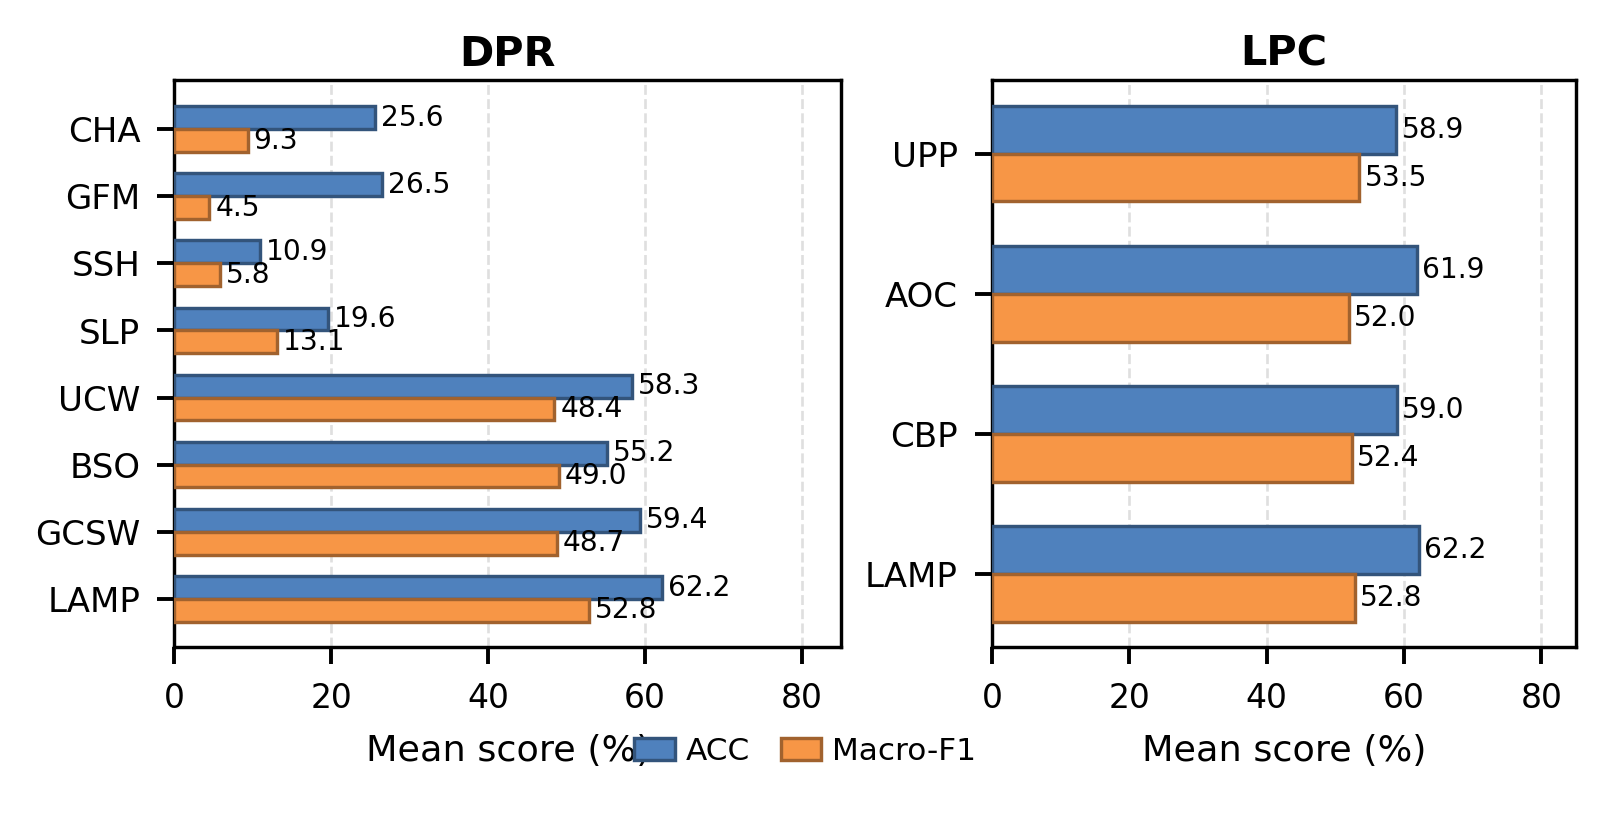
\includegraphics[width=\columnwidth]{figures/02_internal_module_ablations.png}
    \caption{Internal ablations of DPR and LPC. The plotted abbreviations are defined in the ablation text above.}
 
    \label{fig:internal_module_ablations}
\end{figure}

To evaluate LPC, we retain DPR and compare its empirical prior against three controls across the full experimental setting. Uniform prevalence prior (UPP) replaces the measured class distribution with a flat prior, testing whether calibration should ignore observed prevalence altogether. Always-on calibration (AOC) removes the long-tail activation gate so the prior is applied to every configuration, testing whether the gate is a useful safeguard against calibrating near-balanced cases. Client-balanced prior (CBP) estimates the prior by averaging each client's normalized prevalence with equal weight, testing whether equal client influence can replace a sample-count-weighted prevalence estimate.

Table~\ref{tab:prevalence-internal-ablation} and Fig.~\ref{fig:internal_module_ablations} show that LAMP-Merge is best and every control reduces ACC. This demonstrates that calibrated empirical prevalence and client-size-aware aggregation complement DPR.

\begin{figure}[!t]
\centering
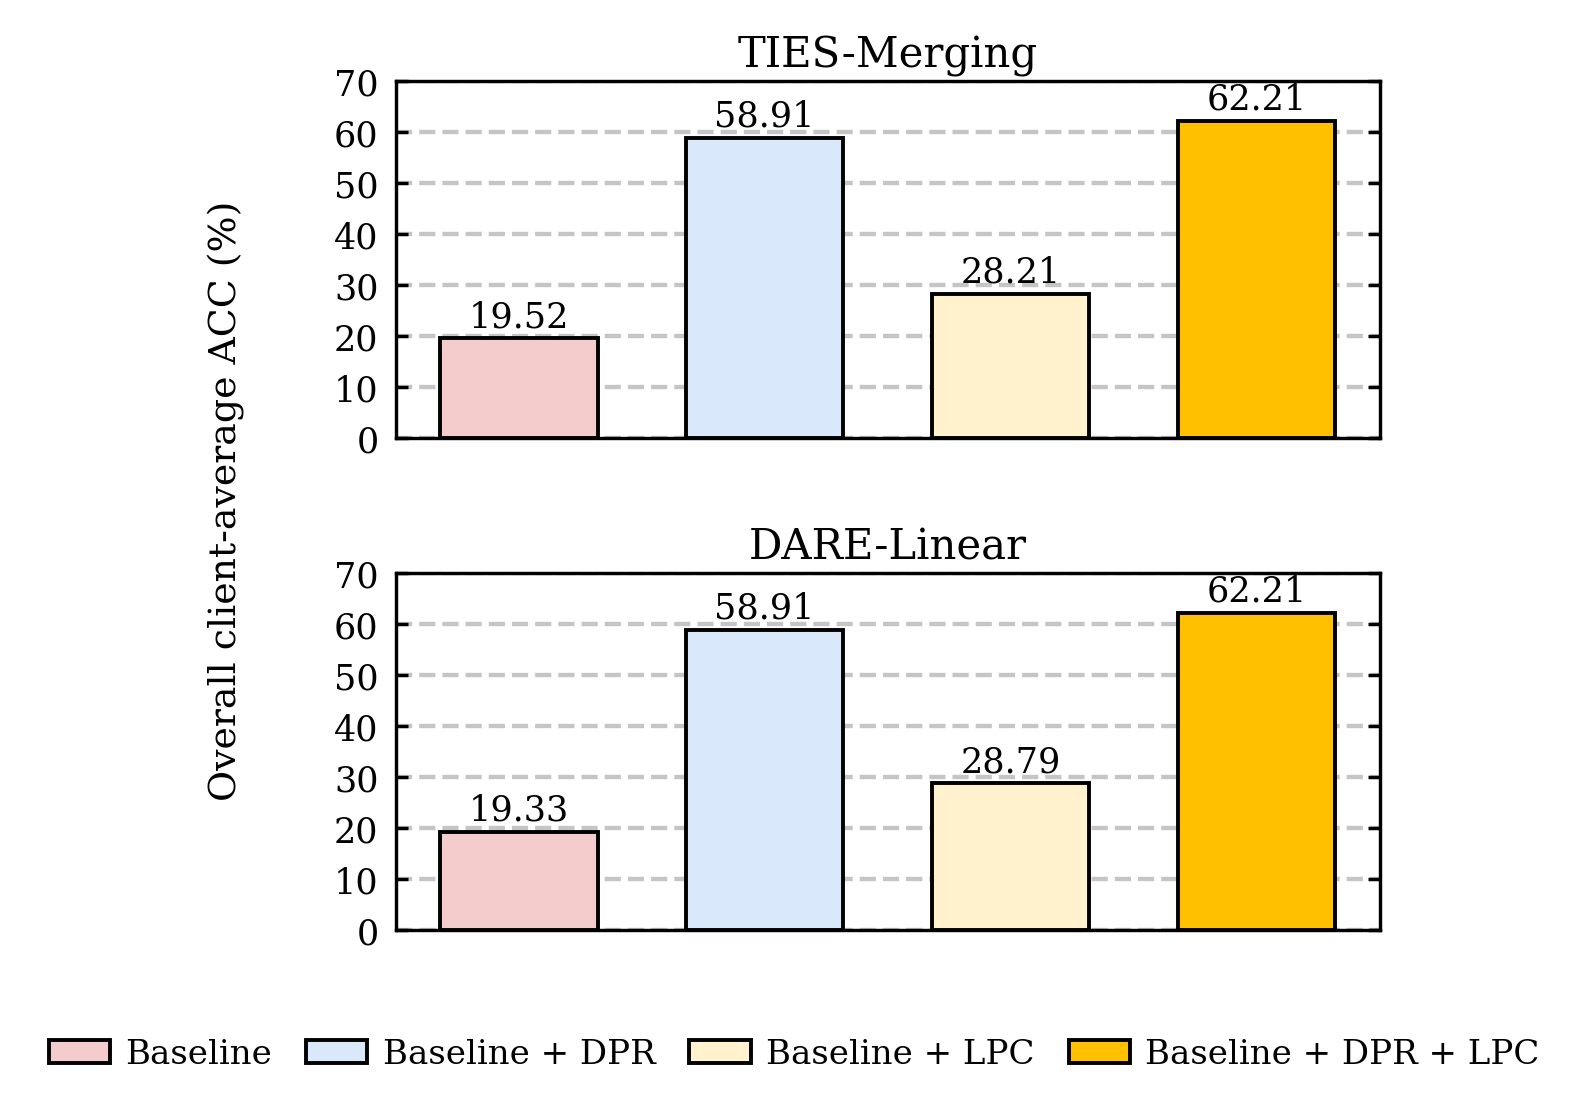
\includegraphics[width=\columnwidth]{figures/03_baseline_2x2_ablation.png}
\caption{Strict $2\times2$ DPR/LPC ablations for TIES-Merging and DARE-Linear. \textbf{All experimental datasets are included.}}
\label{fig:baseline-2x2-ablation}
\end{figure}

\subsection{Innovative prediction-collapse Diagnostics}
Because raw ACC can hide single-class predictions on long-tailed data, we additionally report collapse ratio, effective predicted classes, and predicted--true total variation\cite{BUDA2018249,5597285}. With $q_c$ and $\bar{q}_c$ the predicted and true class distributions over the test set, the three diagnostics are
\begin{equation}
\begin{array}{c}
\rho=\max_c q_c,\qquad C_{\mathrm{eff}}=\exp\left(-\sum_c q_c\log q_c\right),\\[3pt]
\mathrm{TV}(q,\bar{q})=\frac{1}{2}\sum_c|q_c-\bar{q}_c|.
\end{array}
\end{equation}
Lower $\rho$ and TV and higher $C_{\mathrm{eff}}$ indicate weaker prediction collapse.

\begin{table}[!t]
\centering
\caption{Prediction-collapse diagnostics by dataset. Best ref. is selected separately for each metric and dataset. Ratio metrics use percentage scale; Avg averages the five datasets.}
\label{tab:collapse-key}
\scriptsize
\setlength{\tabcolsep}{2.2pt}
\renewcommand{\arraystretch}{1.16}
\resizebox{\columnwidth}{!}{%
\begin{tabular}{clccccc:c}
\noalign{\hrule height 1.25pt}
\rowcolor[HTML]{F2F2F2}
\textbf{Metric} & \textbf{Series} & \textbf{Blood} & \textbf{Derma} & \textbf{Organ-C} & \textbf{Organ-S} & \textbf{US} & \textbf{Avg} \\
\hline \hline
 & \cellcolor{gray!10}Best ref. & \cellcolor{gray!10}80.20 & \cellcolor{gray!10}85.18 & \cellcolor{gray!10}72.38 & \cellcolor{gray!10}71.12 & \cellcolor{gray!10}80.31 & \cellcolor{gray!10}79.02 \\
\multirow{-2}{*}{Collapse $\downarrow$} & \cellcolor[HTML]{FFF9C4}\textbf{LAMP} & \cellcolor[HTML]{FFF9C4}\textbf{19.58} & \cellcolor[HTML]{FFF9C4}\textbf{68.05} & \cellcolor[HTML]{FFF9C4}\textbf{20.72} & \cellcolor[HTML]{FFF9C4}\textbf{24.36} & \cellcolor[HTML]{FFF9C4}\textbf{20.45} & \cellcolor[HTML]{FFF9C4}\textbf{30.63} \\
\hdashline
 & \cellcolor{gray!10}Best ref. & \cellcolor{gray!10}1.81 & \cellcolor{gray!10}1.65 & \cellcolor{gray!10}2.49 & \cellcolor{gray!10}2.53 & \cellcolor{gray!10}1.98 & \cellcolor{gray!10}2.05 \\
\multirow{-2}{*}{Eff. classes $\uparrow$} & \cellcolor[HTML]{FFF9C4}\textbf{LAMP} & \cellcolor[HTML]{FFF9C4}\textbf{7.48} & \cellcolor[HTML]{FFF9C4}\textbf{3.10} & \cellcolor[HTML]{FFF9C4}\textbf{9.55} & \cellcolor[HTML]{FFF9C4}\textbf{8.44} & \cellcolor[HTML]{FFF9C4}\textbf{7.44} & \cellcolor[HTML]{FFF9C4}\textbf{7.20} \\
\hdashline
 & \cellcolor{gray!10}Best ref. & \cellcolor{gray!10}73.48 & \cellcolor{gray!10}46.03 & \cellcolor{gray!10}75.42 & \cellcolor{gray!10}73.85 & \cellcolor{gray!10}72.73 & \cellcolor{gray!10}69.44 \\
\multirow{-2}{*}{Pred-true TV $\downarrow$} & \cellcolor[HTML]{FFF9C4}\textbf{LAMP} & \cellcolor[HTML]{FFF9C4}\textbf{3.97} & \cellcolor[HTML]{FFF9C4}\textbf{17.09} & \cellcolor[HTML]{FFF9C4}\textbf{12.38} & \cellcolor[HTML]{FFF9C4}\textbf{13.17} & \cellcolor[HTML]{FFF9C4}\textbf{15.51} & \cellcolor[HTML]{FFF9C4}\textbf{12.42} \\
\noalign{\hrule height 1.25pt}
\end{tabular}
}
\end{table}

Table~\ref{tab:collapse-key} shows that \textbf{LAMP-Merge consistently improves all collapse diagnostics}.

\subsection{Visualization Experiment}

We visualize the absolute per-class predicted--true gap; values closer to zero indicate better prevalence alignment.

\begin{figure}[!t]
\centering
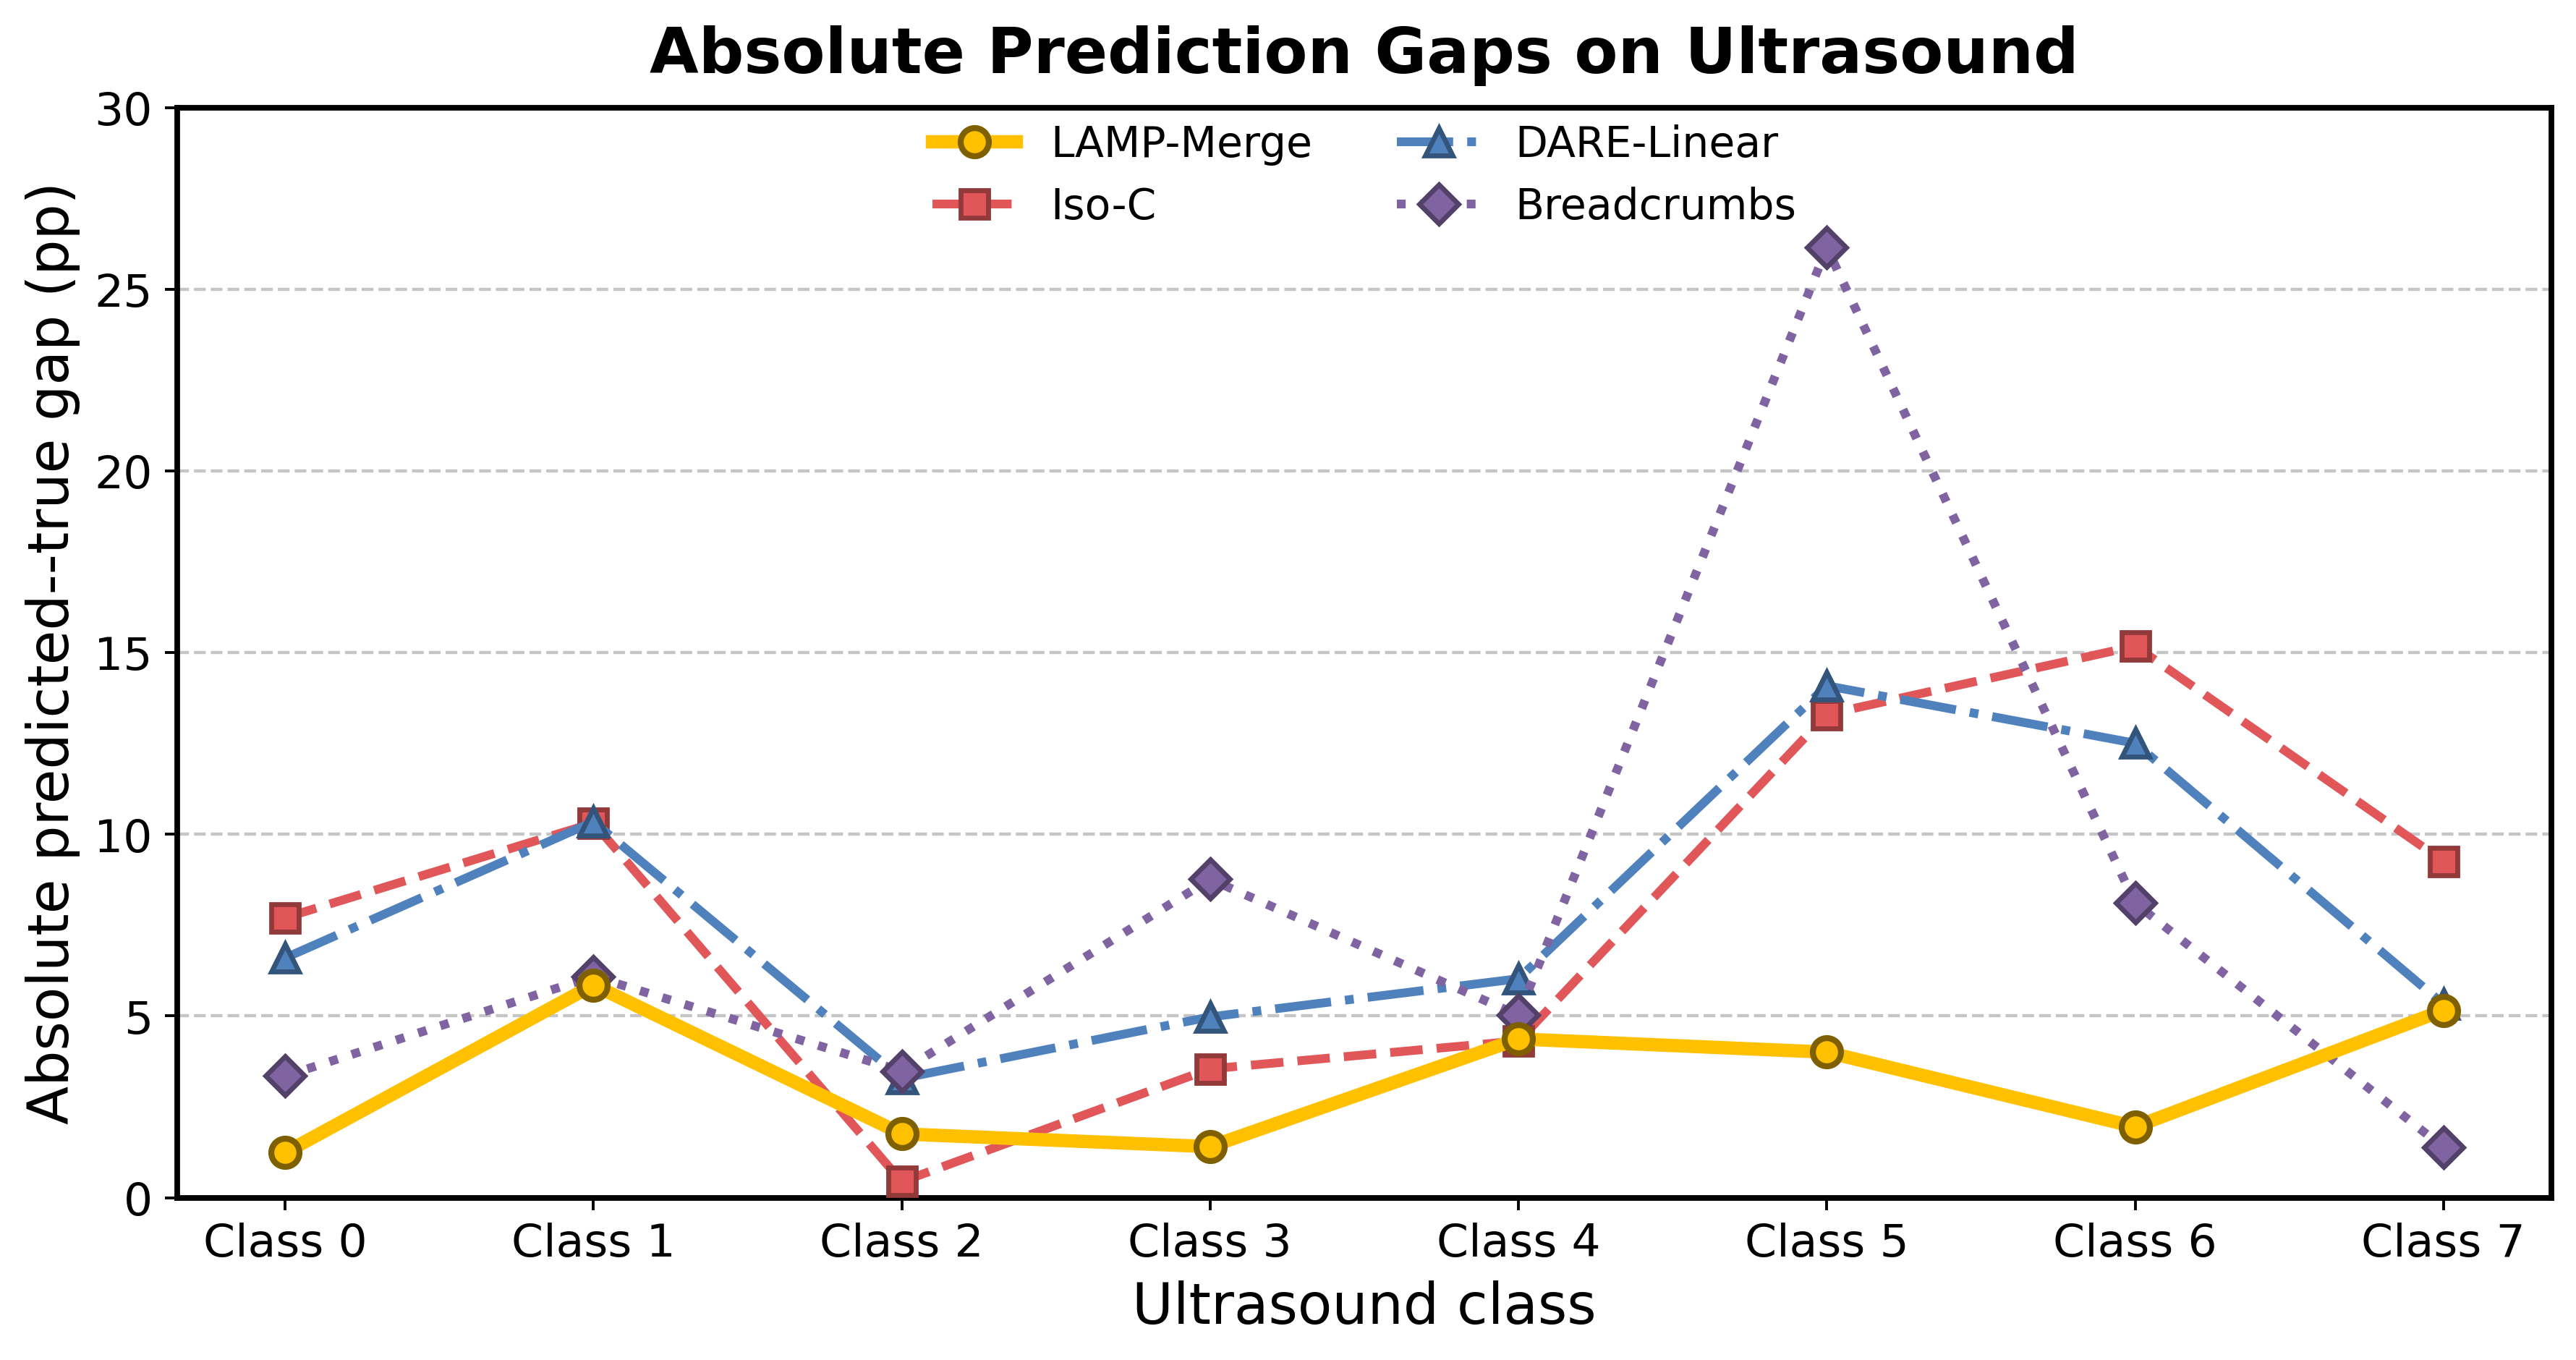
\includegraphics[width=\linewidth]{figures/04_ultrasound_class_distribution.png}
\caption{Absolute predicted--true class gaps on Ultrasound, averaged over all backbones, client counts, and Dirichlet settings. Values are percentage points; zero denotes exact agreement.}
\label{fig:visual-chaosheng_predict}
\end{figure}

\subsection{Hyperparameter Analysis Experiment}
Fig.~\ref{fig:hparam-analysis} evaluates DPR/LPC sensitivity on \textbf{the full setting}.

\begin{figure}[!t]
\centering
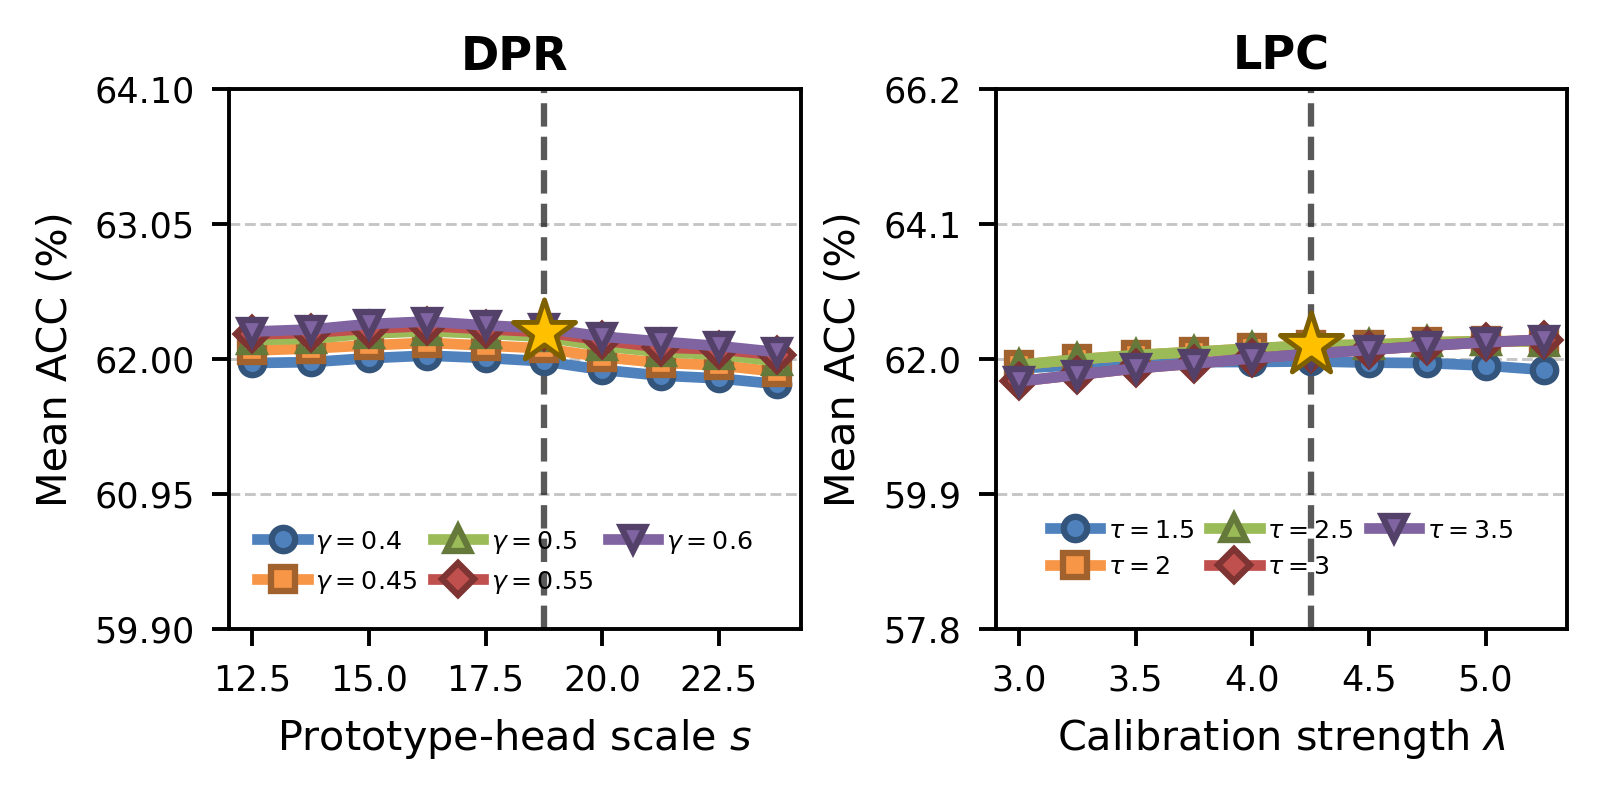
\includegraphics[width=\columnwidth]{figures/05_hyperparameter_sensitivity.png}
\caption{Single-factor DPR/LPC ablation on \textbf{the full setting}; each curve varies one module parameter while all others remain fixed.}
\label{fig:hparam-analysis}
\end{figure}

This single-factor ablation varies DPR's prototype-head scale \(s\) under several \(\gamma\) values and LPC's calibration strength \(\lambda\) under several \(\tau\) values, while holding all remaining settings fixed. The selected \(s=18.75\) lies in a broad high-performing DPR region, and the closely spaced LPC curves around \(\tau=2.5\) show gradual sensitivity rather than an isolated peak.


\section{Conclusion}

We study one-shot medical model merging without raw-image sharing or federated rounds. Under incomplete local coverage, generic merges can collapse predictions, while raw ACC may conceal failure on long-tailed data. Across full-scope experiments, DPR restores class-level directions and LPC retains clinically meaningful prevalence without reintroducing collapse. Together, they offer a class-level interface for privacy-constrained collaboration.

\bibliography{aaai2026}
% \appendix
% \def\appendixinmain{}
% \section{Supplementary Results and Analysis}
\FloatBarrier

\subsection{Detailed Dataset Description}
\label{app:datasets}

The experiments use five MedMNIST v2 benchmarks~\cite{yang2023medmnist}. They were selected to cover microscopy, dermoscopy, CT, and ultrasound while varying the number of diagnostic classes and the prevalence profile. Table~\ref{tab:dataset-statistics} reports the exact split sizes used by the experiments; the descriptions below clarify the recognition problem represented by each benchmark.

\paragraph{Blood.} BloodMNIST is an eight-class microscopy benchmark for recognizing peripheral blood-cell morphology. Its classes include granulocytes, lymphocytes, and other cells with visually similar staining patterns. Fine-grained morphology makes it a useful stress test for whether a merged classifier preserves class-specific directions rather than concentrating its predictions on a small subset of cells.

\paragraph{Derma.} DermaMNIST contains seven dermoscopic skin-lesion categories. Its prevalence is strongly imbalanced and several categories share colour and texture patterns. This setting tests whether a merger distinguishes rare lesions without erasing the clinically meaningful prevalence of common lesions.

\paragraph{Organ-C and Organ-S.} OrganCMNIST and OrganSMNIST provide 11-way abdominal CT organ recognition in coronal and sagittal views, respectively. The two views share the same broad task but change the visible anatomy and image geometry, testing robustness across CT planes.

\paragraph{Ultrasound.} UltrasoundMNIST is an eight-class ultrasound-structure benchmark. Speckle noise, low contrast, and view-dependent boundaries make it particularly suitable for the prediction-collapse diagnostics and the per-class gap visualization in Fig.~\ref{fig:visual-chaosheng_predict}.

\begin{center}
\captionof{table}{BloodMNIST label space used in the experiments. The class IDs agree with the labels in the benchmark NPZ file.}
\label{tab:blood-labels}
\small
\renewcommand{\arraystretch}{1.12}
\begin{tabular}{clcl}
\noalign{\hrule height 1.25pt}
\rowcolor[HTML]{F2F2F2}
\textbf{ID} & \textbf{Class} & \textbf{ID} & \textbf{Class} \\
\hline \hline
0 & Basophil & 4 & Lymphocyte \\
\rowcolor{gray!10}
1 & Eosinophil & 5 & Monocyte \\
2 & Erythroblast & 6 & Neutrophil \\
\rowcolor{gray!10}
3 & Immature granulocyte & 7 & Platelet \\
\noalign{\hrule height 1.25pt}
\end{tabular}
\end{center}

\begin{figure*}[!t]
\centering
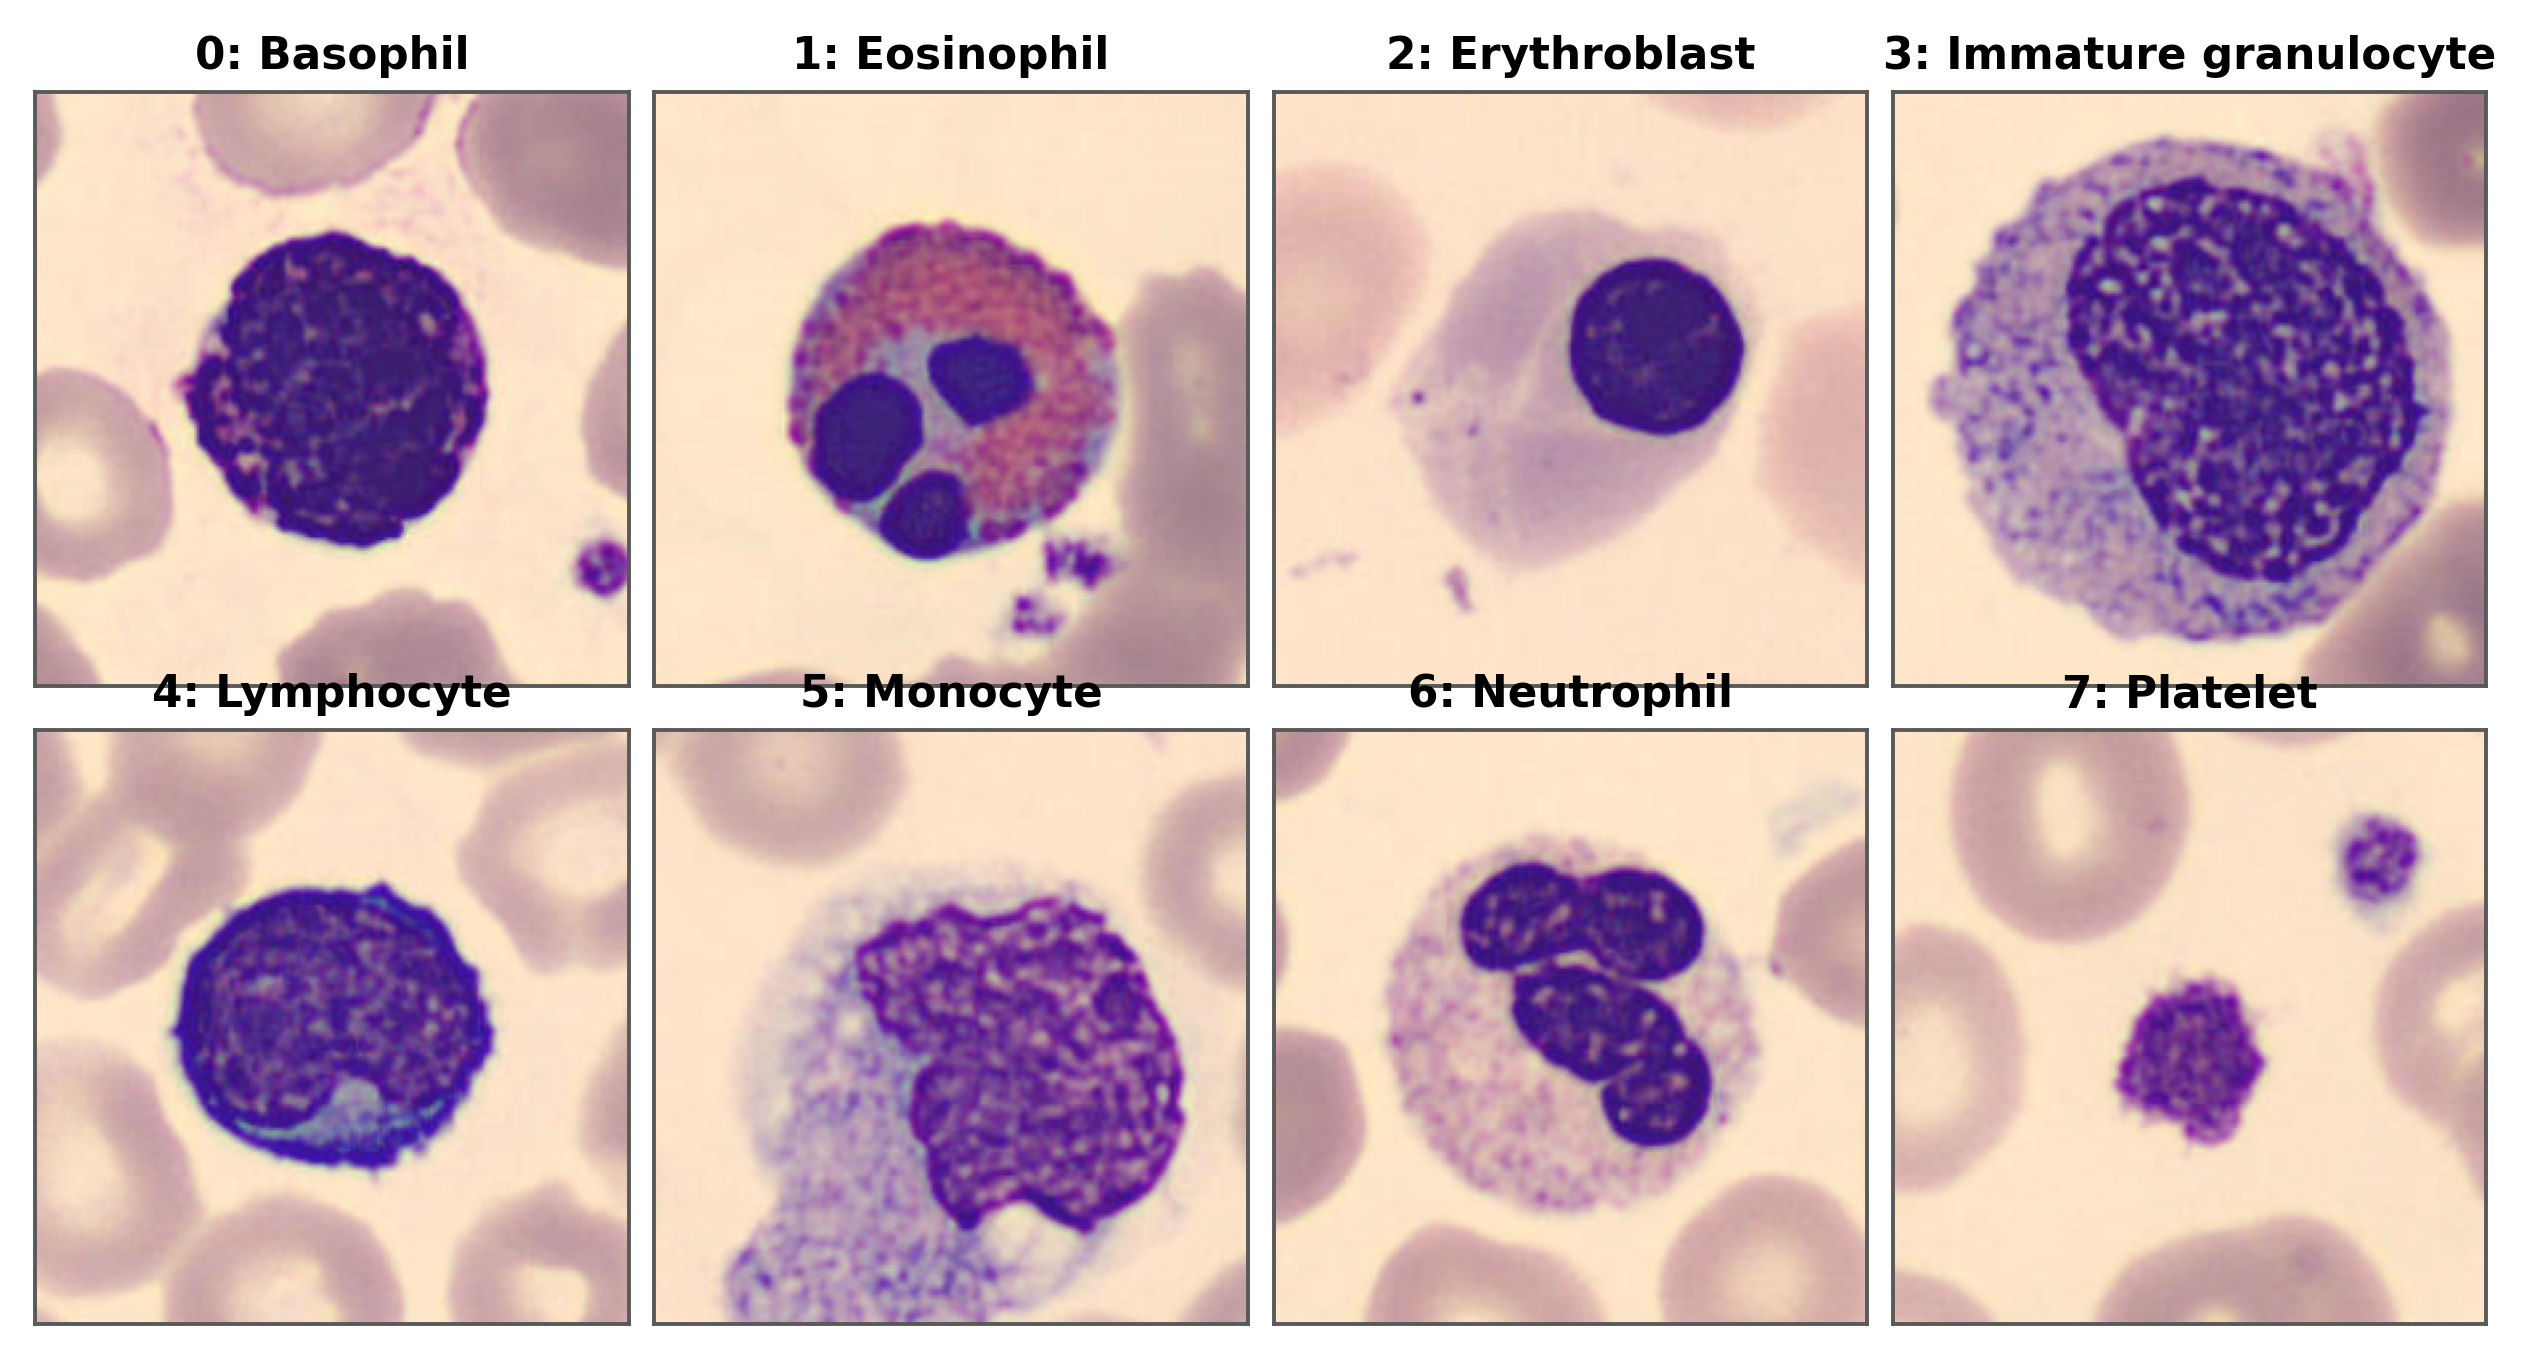
\includegraphics[width=0.93\textwidth]{figures/appendix_blood_classes.png}
\caption{Representative BloodMNIST training examples, one for every class in Table~\ref{tab:blood-labels}. Images are drawn directly from the labeled benchmark file used to construct the experimental partitions; they are shown only to document class appearance, not as training data for merging.}
\label{fig:blood-class-reference}
\end{figure*}

\subsection{Detailed Ablation Configurations and Interpretation}
\label{app:ablation-configurations}

All internal ablations use the same five datasets, four backbones, client counts, and Dirichlet settings as the main experiment. Thus, a change in Table~\ref{tab:diagnostic-internal-ablation} or Table~\ref{tab:prevalence-internal-ablation} isolates one design choice while holding the remaining LAMP-Merge pipeline fixed.

\subsubsection{Diagnostic Prototype Reconstruction}

For class \(c\), DPR aggregates reference-space prototypes as
\begin{equation}
p_c=\sum_{i=1}^{K}\alpha_{i,c}\mu_{i,c},\qquad
\alpha_{i,c}=\frac{e_{i,c}}{\sum_j e_{j,c}}.
\label{eq:appendix-dpr}
\end{equation}
\begin{equation}
e_{i,c}=(n_{i,c}+1)^\gamma\mathbf{1}[n_{i,c}>0].
\end{equation}
Here \(\mu_{i,c}\) is client \(i\)'s class-conditional reference-space mean and \(n_{i,c}\) is its support for that class. The substitutions below test whether the class semantics in \(\mu_{i,c}\) and the class-specific reliability in \(\alpha_{i,c}\) are both required.

\paragraph{Classifier-head aggregation (CHA).} CHA replaces the reference-space evidence by the local classifier-head direction, \(\mu_{i,c}\leftarrow h_{i,c}\). It tests whether client heads already provide a common, class-aligned representation. Its mean ACC is 25.63\%, a 36.58-point reduction from LAMP-Merge (62.21\%), showing that independently trained head directions are not a reliable substitute for shared-space class evidence.

\paragraph{Global-feature mean (GFM).} GFM removes class conditioning by using the same class-agnostic feature mean for every class, \(\mu_{i,c}\leftarrow g\). This tests whether generic client appearance alone can drive merging. Its 26.50\% mean ACC is 35.71 points below LAMP-Merge, indicating that class conditioning, not merely feature aggregation, is essential.

\paragraph{Support-only synthetic head (SSH).} SSH removes image-derived prototype information and sets \(p_c\leftarrow u_c\), where \(u_c\) is a fixed random unit vector. It preserves the classifier interface while eliminating diagnostic content. The 10.89\% mean ACC, 51.32 points below LAMP-Merge, verifies that performance does not arise from support counts or the cosine-head form alone.

\paragraph{Shuffled-label prototype (SLP).} SLP preserves prototype magnitudes but destroys their label correspondence, \(p_c\leftarrow p_{\sigma(c)}\), for a permutation \(\sigma\) of the diagnosis labels. Its 19.57\% mean ACC (a 42.64-point reduction) directly tests semantic alignment: useful class evidence must be assigned to the correct output class.

\paragraph{Uniform client weight (UCW).} UCW retains class prototypes but weights every client observing \(c\) equally:
\begin{equation}
\alpha_{i,c}\leftarrow\frac{\mathbf{1}[n_{i,c}>0]}{\sum_j\mathbf{1}[n_{j,c}>0]}.
\end{equation}
It tests whether observing a class is sufficient, independent of the amount of evidence. Its 58.33\% mean ACC is 3.88 points below LAMP-Merge, showing that support magnitude provides useful reliability information beyond class presence.

\paragraph{Binary support only (BSO).} BSO turns both prototype support and prevalence counts into presence indicators, \(n_{i,c},m_{i,c}\leftarrow\mathbf{1}[n_{i,c}>0]\). It tests whether fine-grained class frequency is necessary in both modules. The mean ACC falls to 55.18\% (7.03 points below LAMP-Merge), the largest loss among the weighting controls.

\paragraph{Global client-size weight (GCSW).} GCSW replaces class-specific reliability by total client size, \(e_{i,c}\leftarrow(N_i+1)^\gamma\mathbf{1}[n_{i,c}>0]\), where \(N_i=\sum_k n_{i,k}\). It tests whether a generally large client can stand in for strong evidence of a particular class. Its 59.39\% mean ACC, 2.82 points below LAMP-Merge, shows that local data volume should be assigned at the class level.

\paragraph{DPR summary.} The semantic controls cause large reductions (35.71--51.32 points), while the weighting controls cause smaller but consistent reductions (2.82--7.03 points). Together, these results support the two parts of Eq.~\ref{eq:appendix-dpr}: class-conditioned shared-space evidence provides the discriminative direction, and class-specific support determines how reliably each client contributes to that direction.

\subsubsection{Long-tail Prevalence Calibration}

LPC estimates an empirical prior and adds a centered, gated log-prior bias after DPR:
\begin{equation}
\pi_c=\frac{\sum_i m_{i,c}}{\sum_k\sum_i m_{i,k}},\qquad
b_c=\lambda\left(\log\pi_c-\frac{1}{C}\sum_k\log\pi_k\right).
\label{eq:appendix-lpc}
\end{equation}
\begin{equation}
\ell_c(x)=w_c^\top\phi_0(T(x))+\mathbf{1}[r>\tau]b_c.
\end{equation}
The three controls retain DPR and test the prior estimator or the activation gate in Eq.~\ref{eq:appendix-lpc}.

\paragraph{Uniform prevalence prior (UPP).} UPP suppresses prevalence information by setting \(\pi_c\leftarrow1/C\). It tests whether calibration should ignore the observed class distribution. Mean ACC is 58.91\%, 3.30 points below LAMP-Merge, demonstrating that the empirical prior is useful rather than a source of collapse.

\paragraph{Always-on calibration (AOC).} AOC removes the long-tail criterion and sets \(\mathbf{1}[r>\tau]\leftarrow1\). It tests whether the prior should be applied uniformly to every configuration. Its 61.90\% mean ACC is 0.31 points below LAMP-Merge. The small aggregate gap indicates that calibration is broadly useful, while the gated design avoids imposing a prior when a configuration is not sufficiently long-tailed.

\paragraph{Client-balanced prior (CBP).} CBP gives every client equal prior influence:
\begin{equation}
\pi_c\leftarrow\frac{1}{K}\sum_i\frac{m_{i,c}}{\sum_k m_{i,k}}.
\end{equation}
It tests whether each client should contribute equally regardless of sample volume. The 58.97\% mean ACC, 3.24 points below LAMP-Merge, favors the sample-count empirical prior over a client-balanced estimate.

\paragraph{LPC summary.} Every LPC control is below the 62.21\% LAMP-Merge mean. UPP and CBP show that both prevalence information and its sample-size weighting matter; AOC shows that the activation criterion is a targeted safeguard rather than the primary source of the gain. Hence LPC calibrates DPR's restored class directions instead of replacing them with a prior.

\subsection{Additional Analysis of DPR and LPC}

\subsubsection{Prototype estimation and class margins}

Let \(\mu_c^\star\) be the population class mean in the shared reference space. For client-level class estimates with bounded second moments, the mean-squared error of the aggregated prototype obeys
\begin{equation}
\mathrm{E}\|p_c-\mu_c^\star\|_2^2
\leq\sum_i\alpha_{i,c}^2\frac{\sigma_c^2}{n_{i,c}}+\mathrm{Bias}_c^2.
\label{eq:prototype-bound}
\end{equation}
The first term is a variance contribution: it decreases with support \(n_{i,c}\), but only clients that observed class \(c\) may contribute. The second term represents systematic mismatch between a local class estimate and the shared-space population mean. Equation~\ref{eq:prototype-bound} explains both support-related controls: UCW ignores unequal estimation variance, whereas GCSW confuses total client size with the support relevant to class \(c\).

For a reference feature \(z=\phi_0(T(x))\), consider two candidate classes \(c\) and \(d\). The population margin is
\begin{equation}
\Delta_{c,d}(x)=(\mu_c^\star)^\top z-(\mu_d^\star)^\top z.
\end{equation}
If
\begin{equation}
\|p_c-\mu_c^\star\|_2+\|p_d-\mu_d^\star\|_2
<\frac{\Delta_{c,d}(x)}{\|z\|_2},
\label{eq:margin-condition}
\end{equation}
then the reconstructed prototypes preserve the ordering between \(c\) and \(d\). Thus, class-specific aggregation is not intended to reproduce arbitrary local heads: it reduces prototype error sufficiently to retain discriminative class margins. The large losses for CHA, GFM, SSH, and SLP are consistent with breaking precisely this semantic margin mechanism.

\subsubsection{Bounded prevalence correction}

The centering in Eq.~\ref{eq:appendix-lpc} removes the uniform component of the log prior. Therefore only relative scores change, with
\begin{equation}
b_c-b_d=\lambda\log\frac{\pi_c}{\pi_d}.
\end{equation}
The gate \(\mathbf{1}[r>\tau]\) applies this relative correction only under sufficient prevalence imbalance, and the finite \(\lambda\) bounds its magnitude. DPR consequently supplies the class directions, while LPC adjusts the decision boundary only when the empirical class prevalence provides relevant evidence. This division also explains why a prevalence-only mechanism cannot solve the semantic controls in Table~\ref{tab:diagnostic-internal-ablation}.

\subsection{Metric Definitions}
\label{app:metric-geometry}

Let \(y_n\) and \(\hat{y}_n\) denote the true and predicted labels of sample \(n\), respectively. Let \(q_c=N^{-1}\sum_n\mathbf{1}[\hat{y}_n=c]\) be the predicted class distribution and \(p_c=N^{-1}\sum_n\mathbf{1}[y_n=c]\) the true distribution. The prediction-collapse diagnostics are
\begin{equation}
\rho=\max_c q_c,\qquad
C_{\mathrm{eff}}=\exp\left(-\sum_cq_c\log q_c\right).
\end{equation}
\begin{equation}
\mathrm{TV}(q,p)=\frac{1}{2}\sum_c|q_c-p_c|.
\end{equation}
The collapse ratio \(\rho\) measures the largest predicted-class share, \(C_{\mathrm{eff}}\) measures the effective number of classes used by the predictor, and TV measures distributional disagreement with the labels. Lower \(\rho\) and TV and higher \(C_{\mathrm{eff}}\) are preferred. The absolute per-class gaps in Fig.~\ref{fig:visual-chaosheng_predict} are \(|q_c-p_c|\) in percentage points and expose which classes contribute to TV.

\subsection{Hyperparameter-Sweep Reproducibility}

Every point in Fig.~\ref{fig:hparam-analysis} is a completed full-configuration experiment covering five datasets, four backbones, three client counts, and three Dirichlet settings (180 raw cells, or 60 client-average cells after averaging the three skew levels). The plotted curves retain measured points in ascending parameter order; no smoothing, interpolation, or best-run selection is applied. The LPC grid records \(\tau\in\{2.0,2.5,3.0\}\) and calibration strengths \(\lambda\in\{3.00,3.25,\ldots,5.25\}\), with \(\gamma=0.55\) and \(s=18.75\) fixed. DPR completion records are read from the full-configuration run directories and are plotted only after all 180 cells have succeeded. The selected operating point is \(\gamma=0.55\), \(s=18.75\), \(\tau=2.5\), and \(\lambda=4.25\), making its reported value traceable to the same completed grid as its neighboring points.


\end{document}
